\documentclass[degree=bachelor,language=english,tocarialchapter]{thuthesis}
% 选项
%   degree=[bachelor|master|doctor|postdoctor], % 必选,学位类型
%   language=[chinese|english], % 可选(默认:chinese),论文的主要语言
%   secret,                % 可选(默认:关闭),是否有密级
%   tocarialchapter,       % 可选(默认:关闭),章目录中使用黑体(这项表示同时打开下面两项)
%   tocarialchapterentry,  % 可选(默认:关闭),单独控制章标题在目录中使用黑体
%   tocarialchapterpage,   % 可选(默认:关闭),单独控制章页码在目录中使用黑体

% 所有其它可能用到的包都统一放到这里了,可以根据自己的实际添加或者删除。
\usepackage{thuthesis}

% 定义所有的图片文件在 figures 子目录下
\graphicspath{{figures/}}

% ----------------------------------------------------------------------
%           Alphabetical Shortcut Table
% ----------------------------------------------------------------------

\newcommand*\widefbox[1]{\fbox{\hspace{2em}#1\hspace{2em}}}
\newcommand{\xint}{\int_{x_1}^{x_2}}
\newcommand{\tint}{\int_{t_1}^{t_2}}
\newcommand{\mw}{\sqrt{m\omega}}
\newcommand{\de}{\delta}
\newcommand{\dde}{\dot{\delta}}
\newcommand{\di}{\delta_i}
\newcommand{\ddi}{\dot{\delta_i}}
\newcommand{\dddi}{\ddot{\delta_i}}
\newcommand{\dipl}{\delta_{i+1}}
\newcommand{\dimi}{\delta_{i-1}}
\newcommand{\ddt}[1]{\frac{{d} #1}{dt}}
\newcommand{\ddtt}[1]{\frac{d^2 #1}{dt^2}}
\newcommand{\ddx}[1]{\frac{d #1}{dx}}
\newcommand{\ddxx}[1]{\frac{d^2 #1}{dx^2}}
\newcommand{\eps}{\epsilon}
\newcommand{\del}[2]{\frac{\partial #1}{\partial #2}}
\newcommand{\deltwo}[2]{\frac{\partial^2 #1}{\partial #2^2}}
\newcommand{\lam}{\lambda}
\newcommand{\Lam}{\Lambda}
\newcommand{\sig}{\sigma}
\newcommand{\Sig}{\Sigma}
\newcommand{\half}{\frac{1}{2}}
\newcommand{\munu}{{\mu\nu}}
\newcommand{\thalf}{\tfrac{1}{2}}

\newcommand{\bfA}{{\bf A}}
\newcommand{\bfB}{{\bf B}}
\newcommand{\bfC}{{\bf C}}
\newcommand{\bfD}{{\bf D}}
\newcommand{\bfE}{{\bf E}}
\newcommand{\bfF}{{\bf F}}
\newcommand{\bfG}{{\bf G}}
\newcommand{\bfH}{{\bf H}}
\newcommand{\bfI}{{\bf I}}
\newcommand{\bfJ}{{\bf J}}
\newcommand{\bfK}{{\bf K}}
\newcommand{\bfL}{{\bf L}}
\newcommand{\bfM}{{\bf M}}
\newcommand{\bfN}{{\bf N}}
\newcommand{\bfO}{{\bf O}}
\newcommand{\bfP}{{\bf P}}
\newcommand{\bfQ}{{\bf Q}}
\newcommand{\bfR}{{\bf R}}
\newcommand{\bfS}{{\bf S}}
\newcommand{\bfT}{{\bf T}}
\newcommand{\bfU}{{\bf U}}
\newcommand{\bfV}{{\bf V}}
\newcommand{\bfW}{{\bf W}}
\newcommand{\bfX}{{\bf X}}
\newcommand{\bfY}{{\bf Y}}
\newcommand{\bfZ}{{\bf Z}}

\newcommand{\bfa}{{\bf a}}
\newcommand{\bfb}{{\bf b}}
\newcommand{\bfc}{{\bf c}}
\newcommand{\bfd}{{\bf d}}
\newcommand{\bfe}{{\bf e}}
\newcommand{\bff}{{\bf f}}
\newcommand{\bfg}{{\bf g}}
\newcommand{\bfh}{{\bf h}}
\newcommand{\bfi}{{\bf i}}
\newcommand{\bfj}{{\bf j}}
\newcommand{\bfk}{{\bf k}}
\newcommand{\bfl}{{\bf l}}
\newcommand{\bfm}{{\bf m}}
\newcommand{\bfn}{{\bf n}}
\newcommand{\bfo}{{\bf o}}
\newcommand{\bfp}{{\bf p}}
\newcommand{\bfq}{{\bf q}}
\newcommand{\bfr}{{\bf r}}
\newcommand{\bfs}{{\bf s}}
\newcommand{\bft}{{\bf t}}
\newcommand{\bfu}{{\bf u}}
\newcommand{\bfv}{{\bf v}}
\newcommand{\bfw}{{\bf w}}
\newcommand{\bfx}{{\bf x}}
\newcommand{\bfy}{{\bf y}}
\newcommand{\bfz}{{\bf z}}

\newcommand{\mcA}{{\mathcal{A}}}
\newcommand{\mcB}{{\mathcal{B}}}
\newcommand{\mcC}{{\mathcal{C}}}
\newcommand{\mcD}{{\mathcal{D}}}
\newcommand{\mcE}{{\mathcal{E}}}
\newcommand{\mcF}{{\mathcal{F}}}
\newcommand{\mcG}{{\mathcal{G}}}
\newcommand{\mcH}{{\mathcal{H}}}
\newcommand{\mcI}{{\mathcal{I}}}
\newcommand{\mcJ}{{\mathcal{J}}}
\newcommand{\mcK}{{\mathcal{K}}}
\newcommand{\mcL}{{\mathcal{L}}}
\newcommand{\mcM}{{\mathcal{M}}}
\newcommand{\mcN}{{\mathcal{N}}}
\newcommand{\mcO}{{\mathcal{O}}}
\newcommand{\mcP}{{\mathcal{P}}}
\newcommand{\mcQ}{{\mathcal{Q}}}
\newcommand{\mcR}{{\mathcal{R}}}
\newcommand{\mcS}{{\mathcal{S}}}
\newcommand{\mcT}{{\mathcal{T}}}
\newcommand{\mcU}{{\mathcal{U}}}
\newcommand{\mcV}{{\mathcal{V}}}
\newcommand{\mcW}{{\mathcal{W}}}
\newcommand{\mcX}{{\mathcal{X}}}
\newcommand{\mcY}{{\mathcal{Y}}}
\newcommand{\mcZ}{{\mathcal{Z}}}

\newcommand{\bbA}{{\mathbb{A}}}
\newcommand{\bbB}{{\mathbb{B}}}
\newcommand{\bbC}{{\mathbb{C}}}
\newcommand{\bbD}{{\mathbb{D}}}
\newcommand{\bbE}{{\mathbb{E}}}
\newcommand{\bbF}{{\mathbb{F}}}
\newcommand{\bbG}{{\mathbb{G}}}
\newcommand{\bbH}{{\mathbb{H}}}
\newcommand{\bbI}{{\mathbb{I}}}
\newcommand{\bbJ}{{\mathbb{J}}}
\newcommand{\bbK}{{\mathbb{K}}}
\newcommand{\bbL}{{\mathbb{L}}}
\newcommand{\bbM}{{\mathbb{M}}}
\newcommand{\bbN}{{\mathbb{N}}}
\newcommand{\bbO}{{\mathbb{O}}}
\newcommand{\bbP}{{\mathbb{P}}}
\newcommand{\bbQ}{{\mathbb{Q}}}
\newcommand{\bbR}{{\mathbb{R}}}
\newcommand{\bbS}{{\mathbb{S}}}
\newcommand{\bbT}{{\mathbb{T}}}
\newcommand{\bbU}{{\mathbb{U}}}
\newcommand{\bbV}{{\mathbb{V}}}
\newcommand{\bbW}{{\mathbb{W}}}
\newcommand{\bbX}{{\mathbb{X}}}
\newcommand{\bbY}{{\mathbb{Y}}}
\newcommand{\bbZ}{{\mathbb{Z}}}

\newcommand{\mfa}{{\mathfrak{a}}}
\newcommand{\mfb}{{\mathfrak{b}}}
\newcommand{\mfc}{{\mathfrak{c}}}
\newcommand{\mfd}{{\mathfrak{d}}}
\newcommand{\mfe}{{\mathfrak{e}}}
\newcommand{\mff}{{\mathfrak{f}}}
\newcommand{\mfg}{{\mathfrak{g}}}
\newcommand{\mfh}{{\mathfrak{h}}}
\newcommand{\mfi}{{\mathfrak{i}}}
\newcommand{\mfj}{{\mathfrak{j}}}
\newcommand{\mfk}{{\mathfrak{k}}}
\newcommand{\mfl}{{\mathfrak{l}}}
\newcommand{\mfm}{{\mathfrak{m}}}
\newcommand{\mfn}{{\mathfrak{n}}}
\newcommand{\mfo}{{\mathfrak{o}}}
\newcommand{\mfp}{{\mathfrak{p}}}
\newcommand{\mfq}{{\mathfrak{q}}}
\newcommand{\mfr}{{\mathfrak{r}}}
\newcommand{\mfs}{{\mathfrak{s}}}
\newcommand{\mft}{{\mathfrak{t}}}
\newcommand{\mfu}{{\mathfrak{u}}}
\newcommand{\mfv}{{\mathfrak{v}}}
\newcommand{\mfw}{{\mathfrak{w}}}
\newcommand{\mfx}{{\mathfrak{x}}}
\newcommand{\mfy}{{\mathfrak{y}}}
\newcommand{\mfz}{{\mathfrak{z}}}

\newcommand{\mfA}{{\mathfrak{A}}}
\newcommand{\mfB}{{\mathfrak{B}}}
\newcommand{\mfC}{{\mathfrak{C}}}
\newcommand{\mfD}{{\mathfrak{D}}}
\newcommand{\mfE}{{\mathfrak{E}}}
\newcommand{\mfF}{{\mathfrak{F}}}
\newcommand{\mfG}{{\mathfrak{G}}}
\newcommand{\mfH}{{\mathfrak{H}}}
\newcommand{\mfI}{{\mathfrak{I}}}
\newcommand{\mfJ}{{\mathfrak{J}}}
\newcommand{\mfK}{{\mathfrak{K}}}
\newcommand{\mfL}{{\mathfrak{L}}}
\newcommand{\mfM}{{\mathfrak{M}}}
\newcommand{\mfN}{{\mathfrak{N}}}
\newcommand{\mfO}{{\mathfrak{O}}}
\newcommand{\mfP}{{\mathfrak{P}}}
\newcommand{\mfQ}{{\mathfrak{Q}}}
\newcommand{\mfR}{{\mathfrak{R}}}
\newcommand{\mfS}{{\mathfrak{S}}}
\newcommand{\mfT}{{\mathfrak{T}}}
\newcommand{\mfU}{{\mathfrak{U}}}
\newcommand{\mfV}{{\mathfrak{V}}}
\newcommand{\mfW}{{\mathfrak{W}}}
\newcommand{\mfX}{{\mathfrak{X}}}
\newcommand{\mfY}{{\mathfrak{Y}}}
\newcommand{\mfZ}{{\mathfrak{Z}}}
\usepackage{xcolor}
\renewcommand{\emph}[1]{\textcolor{purple}{\textit{#1}}} % for emph color

\usepackage{siunitx} % \SI{1.234}{\m\per\square\s} \SI{1e-4}{\metre}
\DeclareSIUnit{\rad}{rad} % \rad is removed frmo siunitx 2 since it is not a SI unit. 

% \usepackage{amsmath}
\newcommand\vect{\mathbf}
% \newcommand\matr{\mathbf} % \matrix is defined in LaTeX2e kernel
% \newcommand\tens{\mathcal}

\usepackage{romannum}  % \Romannum{3} \romannum{3}


\def\degree{${}^{\circ}$} % degree symbols
\sisetup{math-micro=\text{µ},text-micro=µ} 
% Very strange that the micro symbol does not appear in \SI{}{}, 
% this is a bug found at https://tex.stackexchange.com/questions/33965/siunitx-µ-doesnt-work 
\usepackage[super]{nth} % 1st, 2nd, ...


% Conflict with thuthesis
% \usepackage[math-style=ISO]{unicode-math} % XeTeX driver only supports unicode.  (hyperref)  Enabling option `unicode'. 
% Sometimes pasted texts may contain unicode math symbols which may cause compiling errors, the package is capable to help you skip those trivial errors caused by compiling those symbols which used to be uncompilable properly.

\usepackage{etoolbox}
\newbool{isBeamer} 
% \booltrue{isBeamer}
\boolfalse{isBeamer}
% \ifbool{isBeamer}{<true>}{<false>}

\usepackage{booktabs}

\makeatletter
\newcommand{\rmnum}[1]{\romannumeral #1}
\newcommand{\Rmnum}[1]{\expandafter\@slowromancap\romannumeral #1@}
\makeatother
\usepackage{hyperref}


% \usepackage[T1]{fontenc} //This may cause some alignment problem in cover
\usepackage[utf8]{inputenc}


% Special scientist naem 
\usepackage{xspace}
\newcommand{\Poincare}{Poincar\'e\xspace}
\newcommand{\adele}{ad\`ele\xspace}
\newcommand{\Cech}{\v{C}ech\xspace}
\newcommand{\Erdos}{Erd\H{o}s\xspace}
\makeatletter
\newcommand{\etale}{\'etal\@ifstar{\'e}{e\xspace}}
\makeatother


\newcommand{\vE}{\vect{E}}
\newcommand{\vx}{\vect{x}}
\newcommand{\vv}{\vect{v}}
\newcommand{\ftxv}{f(t, \vect{x}, \vect{v})}
\newcommand{\bbRRR}{\bbR^{3}}
\newcommand{\bbRx}{\bbR_{x}^{3}}
\newcommand{\bbRv}{\bbR_{v}^{3}}

% 可以在这里修改配置文件中的定义。导言区可以使用中文。
% \def\myname{薛瑞尼}

\begin{document}

%%% 封面部分
\frontmatter
\thusetup{
  %******************************
  % 注意:
  %   1. 配置里面不要出现空行
  %   2. 不需要的配置信息可以删除
  %******************************
  %
  %=====
  % 秘级
  %=====
  % secretlevel={秘密},
  % secretyear={10},
  %
  %=========
  % 中文信息
  %=========
  ctitle={三维扰动场对等离子体边界磁拓扑影响的协同优化模拟},
  cdegree={工学本科},
  cdepartment={工程物理系},
  cmajor={工程物理},
  cauthor={魏文崟},
  csupervisor={梁云峰教授},
  cassosupervisor={高喆教授}, % 副指导老师
  ccosupervisor={高喆教授}, % 联合指导老师
  % 日期自动使用当前时间,若需指定按如下方式修改:
  % cdate={超新星纪元},
  %
  % 博士后专有部分
  % catalognumber     = {},  % 可以留空
  % udc               = {},  % 可以留空
  % id                = {},  % 可以留空: id={},
  % cfirstdiscipline  = {},  % 流动站(一级学科)名称
  % cseconddiscipline = {},  % 专 业(二级学科)名称
  % postdoctordate    = {},  % 工作完成日期
  % postdocstartdate  = {},  % 研究工作起始时间
  % postdocenddate    = {},  % 研究工作期满时间
  %
  %=========
  % 英文信息
  %=========
  etitle={Collaborative Optimization of Multiple 3D Magnetic Perturbation Fields according to Their Effects on Plasma Edge Magnetic Topology in EAST tokamak},
  % 这块比较复杂,需要分情况讨论:
  % 1. 学术型硕士
  %    edegree:必须为Master of Arts或Master of Science(注意大小写)
  %             “哲学、文学、历史学、法学、教育学、艺术学门类,公共管理学科
  %              填写Master of Arts,其它填写Master of Science”
  %    emajor:“获得一级学科授权的学科填写一级学科名称,其它填写二级学科名称”
  % 2. 专业型硕士
  %    edegree:“填写专业学位英文名称全称”
  %    emajor:“工程硕士填写工程领域,其它专业学位不填写此项”
  % 3. 学术型博士
  %    edegree:Doctor of Philosophy(注意大小写)
  %    emajor:“获得一级学科授权的学科填写一级学科名称,其它填写二级学科名称”
  % 4. 专业型博士
  %    edegree:“填写专业学位英文名称全称”
  %    emajor:不填写此项
  edegree={Bachelor of Engineering Physics},
  emajor={Engineering Physics},
  eauthor={Wei, Wenyin},
  esupervisor={Professor Liang, Yunfeng},
  % eassosupervisor={Chen Wenguang},
  % 日期自动生成,若需指定按如下方式修改:
  % edate={December, 2005},
  %
  % 关键词用“英文逗号”分割
  ckeywords={扰动场, 边界局域模, 共振磁扰动, 高 m 线圈, 低杂波, 螺旋电流丝},
  ekeywords={magnetic perturbation field, edge localized mode (ELM), resonant magnetic perturbation (RMP),high m coil, lower-hybrid (LH), helical current filament (HCL)}
}

% 定义中英文摘要和关键字
\begin{cabstract}
  本课题来自目前的先进托卡马克位型所面临的现实问题,尽管参数优良的 \Hmode 等离子体使得聚变达到所需参数目标有了更大的可能性,但同时也带来了新的问题。\Hmode 下等离子体边界高压力梯度和强电流密度蕴含的自由能,引起了边界局域模不稳定性。边界局域模会引起热负荷和粒子流强出现近似周期性的脉冲峰值,而这在 DEMO 堆中是不被允许的。

  为了抑制边界局域模, EAST 上先后测试了共振磁扰动线圈 RMP、高 m 线圈和低杂波驱动的螺旋电流丝,这三种扰动场产生机制有所差异,产生的效果也不尽相同。为了使扰动场相互配合达到最优的弱化乃至抑制边界局域模的效果,对它们在等离子体边界造成的扰动场协同作用的研究是很有必要的。 (1) 低 n 线圈,一般称为 RMP 线圈,布置在腔内,它激发起环向模数为 $n=1,2$ 的扰动场在 \east, \ddd 等托卡马克装置上验证了其抑制边界局域模的效应。 (2) 高 m 线圈,是 EAST 团队近两年实验中的线圈,在等离子体环外加上一组四个的线圈,它的特征是扰动场环向模数 $n$ 分布较宽,极向模数 $m$ 较高,由于一组高 $m$ 线圈只分布在一个极向截面处,扰动场的局域性很强。(3) 低杂波驱动的螺旋电流丝,电流丝的具体物理机制还不甚明晰,但其亦能调节边界磁拓扑。由于低杂波天线不像共振磁扰动线圈在腔内易受到损坏且激发出的螺旋电流丝紧靠边界,它有望在 DEMO 堆及日后商业堆中灵活地调节磁拓扑结构。
  
  第二章便进入本文主体,线圈之间如何配合以能够对等离子体施加合适的磁扰动场,为此对磁扰动场径向分量在边界附近的磁面 Fourier 分析得到的磁谱 $\tilde{b}^1_{mn}$ 和 \Poincare 图是必要的。这一章的主体是通过扰动场之间的配合达到较好的抑制 ELM 及保持芯部等离子体较好约束的效果。进一步在第三章中将讨论不同扰动场的配置下第一壁材料上的热负荷和粒子流分布。尽管主要依赖于对 ELM 的抑制效果来选择磁扰动场,但基于扰动场的热负荷优化分布或时间调制能够给出了一种新的调节视角。%对下一代托卡马克而言,%\Hmode 等离子体会造成难以承受的热流和粒子流,
  % 扰动场可以此提供一种调节手段,避免脉冲式的 ELM 破裂造成的材料损害。

\end{cabstract}

% 如果习惯关键字跟在摘要文字后面,可以用直接命令来设置,如下:
% \ckeywords{\TeX, \LaTeX, CJK, 模板, 论文}

\begin{eabstract}
  The thesis discusses the realistic problem confronted by advanced tokamaks research. Though better confinement is obtained with \Hmode plasma than \Lmode, which makes it possible to achieve the threshold acquired by the fusion energy, new problems are also coming. The free energy stored in the high pressure gradient and strong current density in the edge of confined plasma induces edge localized mode (ELM) instability. ELM may cause too intense transient pulses of heat load and particle flux to sustain, which is not allowable in future tokamaks.

  In order to realize ELM suppression, multiple varieties of perturbation fields have been tested in EAST, \textit{i.e.} resonant magnetic perturbation coils, high $m$ coils and helical current filaments induced by lower hybrid wave. Each of these approaches has advantages and disadvantages. It is necessary to research on the collaborative effect if an optimal ELM suppression effect is anticipated. (1) Low n coils,also known as RMP coils, are distributed inside the vessel to stimulate the perturbant field with dominant toroidal mode number $n=1,2$. Its effect to mitigate or suppress ELM is verified in \east, \ddd tokamaks \textit{etc.}. (2) High m coils are under design by \east team in these two years. Normally four coils are imposed in one poloidal crosssection $\phi=\text{const.}$ with various theta. High $m$ coils have the characteristics that perturbant spectrum distribute widely in toroidal mode number $n$ while relatively high in poloidal mode number $m$. (3)Helical current filanments(HCFs) induced by lower hybrid waves(LHW). LHW is originally designed to drive core plasma current by Landau damping, but experimental evidence shows that there exists helical current filaments in the scrape-off layer (SOF) while LHW system switches on. Because of the fact that LHW antennas are shielded by limiters, therefore not easy to be damaged, and HCFs are close to the plasma edge, it has the potential to modify the magnetic topology near the edge of plasma flexibly in DEMO and next-generation tokamaks.

  Appropriate collaborative coils setup are discussed in chapter two to exert the suitable perturbation field on the plasma, in which the Fourier spectrum $\tilde{b}^1_{mn}$ of the radial component of perturbation field near the edge of plasma and \Poincare plots are necessary to analyze the topology. How to acquire a satisfactory perturbant result, \textit{i.e.} suppress ELM and sustain well confinement of plasma, constitutes the main content of chapter two. Furthermore, the heat load distribution patterns of various perturbant field combinations are analyzed in chapter three. Though we mainly rely on the ELM suppression effect to alter perturbant recipes, the possibility of adjustment of heat load distribution is considered to provide another perspective on the perturbant field. For next generation tokamaks, \Hmode plasma causes unafforable heat flux and particle flux pulses to the plasms-facing components, for which schemes to adjust the heat pattern are required.
\end{eabstract}

% \ekeywords{\TeX, \LaTeX, CJK, template, thesis}

% 如果使用授权说明扫描页,将可选参数中指定为扫描得到的 PDF 文件名,例如:
% \makecover[scan-auth.pdf]
% \makecover

%% 目录
% \tableofcontents

%% 符号对照表
% \begin{denotation}[3cm]
\item[$(R, \phi, Z)$] 磁约束聚变常用柱坐标
\item[$\kappa$] 热导率或者等离子体延伸率,视其上下文而定。
\item[$q, \vect{q}, |\vect{q}|$] $\vect{q}$ 表示热流强度,$|\vect{q}|$ 表其幅值,$q$ 本文中均表示安全系数
\item[$\delta$] 三角变形系数 triangularity
\item[$a, R_0$] 托卡马克装置小半径、大半径  
\item[$\varepsilon$] 环径比 $=a/R_0$ aspect ratio 
\item[ELM] 边界局域模 Edge Localized Mode
\item[RMP] 共振扰动场线圈 Resonant Magnetic Perturbance
\item[ICRH] 离子回旋共振加热 Ion Cyclotron Resonance Heating  
\item[ITER] 国际热核聚变实验堆计划 International Thermonuclear Experimental Reactor 
\item[DEMO] 示范聚变堆 DEMOnstration power plant
\item[SOL] 刮削层 scrape-off layer
\item[HRB] 螺旋辐射带 Helical Radiation Belt  
\item[HCF] 螺旋电流丝 Helical Current Filament
\end{denotation}



% % 也可以使用 nomencl 宏包:

% \printnomenclature[3cm]




%%% 正文部分
\mainmatter
% \chapter{Existence and Uniqueness}
\label{cha:exist-unique}

\chapter*{Reading Note}
Terms marked with \emph{color} mean they are not yet verified.

The Vlasov equation is studied as a governing equation describing the collisionless plasma physics, 
in which the anistropic velocity distribution contributes a significant influence to the dynamics of the system. When coupled with Maxwell equations as the electromagnetism field governing rule, Vlasov is capable to decide the dynamic 
scenario for particle-field interaction, named Vlasov-Maxwell system (VM). Furthermore, under the assumption that the electrostatic force dominates the interaction, magnetic force is omitted and then comes Vlasov-Poisson problem (VP).

\begin{equation}\text { (VP) }\left\{\begin{array}{l}
    \partial_{t} f+a(v) \cdot \nabla_{x} f+\mu \nabla_{x} \phi \cdot \nabla_{v} f=0 \\
    \Delta \phi=\rho(f):=\int_{\mathbb{R}^{3}} f(t, x, v) d v
\end{array}\right.\end{equation}
where, $\mu \in\{+,-\}, a(v) \in\{v, \hat{v}\},$ and $\hat{v}:=v / \sqrt{1+|v|^{2}}$. The sign of $\mu$ indicates different physical scenario, "+" for the plasma physics case and "-" for the stellar dynamics case.

Phase space distribution $\ftxv\geq 0 (x\in \bbRx,v\in\bbRv,t\geq 0) $ with initial datum $f_{0}(\vx, \vv)=f(0, \vx, \vv)$ determines the particle density at $(t, \vx,\vv)$, \textit{i.e.}, the number of particles per unit volumn in phase space.

Some quantities have physical meaning are introduced as follows,
\begin{equation}\begin{array}{c}
    E(t, x)=\nabla_{x} \phi(t, x), \quad \phi=\frac{1}{4 \pi} \frac{1}{|x|} *\rho \\
    \quad \rho(t, x)=\int f(t, x, v) d v, \quad j(t, x)=\int a(v)f(t, x, v) d v
\end{array}\end{equation}

The more realistic equations consider relativistic effect when $a(v)=\hat{v}$ and limit the max velocity the particle can reach, transforming the Vlasov-Poisson to relativistic Vlasov-Poisson (RVP) and the Vlasov-Maxwell to relativistic Vlasov-Maxwell (RVM).
\begin{equation}\label{eq:rvm}\text { (VM) }\left\{\begin{array}{l}
f_{t}+a(v) \cdot \nabla_{x} f+\mu(E+a(v) \times B) \cdot \nabla_{v} f=0 \\
E_{t}=\nabla \times B-j \\
B_{t}=-\nabla \times E \\
\nabla \cdot E=\rho, \quad \nabla \cdot B=0
\end{array}\right.\end{equation}
\\
\\

For classical solutions, it is well known that the existence and
uniqueness result of the Vlasov-Poisson system solution have been presented by Iordanskii \footnote{The paper [16] listed in the reference of \cite{1991InMat.105..415L} is missing, refered as Iordanskii, S.V.: The Cauehy problem for the kinetic equation of plasma. Transl., II. Ser.,
Am. Math. Soc. 35, 351-363 (1964)} in dimension
1, \cite{ukai1978classical} in dimension 2, \cite{bardos1985global} in dimensions
3 for small data. 
The case of (nearly) symmetric data has been treated by \cite{batt1977global}, \cite{wollman1980global}, \cite{horst1981classical}, \cite{schaeffer1987global}. \cite{schaeffer1987global} treated the relativistic case of symmetric data in one paper.


\cite{glassey_symmetric_1985} stated the conservative characteristic of mass and energy, $\|\rho(t,\cdot)\|$ has a bound relying on $\|f_0\|_\infty$ and $\mathscr{E}_0$ in plasma case and proved the existence of global classical spherically symmertric solutions to the Cauchy problem with compact support for the 3D RVP system in the plasma physics case. It turns out that, for the case of stellar dynamics, the "small" data with $40M^{2/3}\|f_0\|_\infty^{1/3}$ will sustain the solution globally while the "large" data for which $-\infty <\mathscr{E}_0<0$, the solution blows up in finite time.

\cite{1991InMat.105..415L}, based on the representation formula built by the characteristic method considering the source term, proves the propagation of moments in $v$ higher than 3.
More precisely, if $|v|^m f_0\in L^1(\bbR^6)\text{ for all }m<m_0,\text{with } m_0> 3$, then we build a solution
of Vlasov-Poisson equations satisfying $|v|^m \ftxv\in L^1(\bbR^6)\text{ for all }m<m_0,\text{with } m_0> 3$ for any $t>0$. Moreover, for $m_0>6$, \emph{Sobolev injections}  deduces that $E\in L^\infty( [0, T]\times \bbRRR )$ for any $t>0$, and,
following Horst \footnote{The paper [14] listed in the reference of \cite{1991InMat.105..415L} is missing, refered as Horst, E.: Global strong solutions of Vlasov's Equation. Necessary and sufficient conditions
for their existence. Partial differential equations. Banach Cent. Publ. 19, 143 153 (1987)}, $f$ is a smooth function if $f_0(x, v)$ is smooth. This improves
a recent result of Pfaffelm6ser \footnote{The paper [19] listed in the reference of \cite{1991InMat.105..415L} is missing, refered as Pfaffelmoser Global classical (footnote from last page) solutions of the Vlasov-Poisson system in three dimensions
for general initial date. (Preprint)} who has shown independently of our work
the existence of a classical solution when )Co is, roughly speaking, Lipschitz
continuous in the space $L_v^{1}(L_x^\infty)$. 


The existence of global solution for the 3D RVM system with finite energy initial data has been investigated extensively by many authors. \cite{glassey1986singularity} deduced the result that the classical solution can be globally
extended with the strong assumption that $f$ has compact support in $v$ for all the time. \cite{staffilani2001fourier} presents a new perspective with Fourier analysis to the study of 3D RVM system and acquired the same result. 
% See also [1, 12, 28] for improvements of this result.

Continuation criterion for the global existence of the Vlasov-Maxwell system
may be a more relaxed condition than assuming the compact support in $v$ assumption. \cite{robert1989largevelocity} proved that, if the initial data decay at rate $|v|^{−7}$ as $|v| \to\infty$ and
the imposed assumption that bound “$\iint_{\bbRRR} |v|f(t, x, v)dv ≤ \text{Constant}$” holds, then the solution extends globall.
% Recently, an interesting new continuation criterion was given by \cite{2016ArRMA.219..445L}, which says that a regular solution can be
% extended as long as k(1+|v|2)θ/2f(t, x, v)kLq xL1 v remains bounded for θ > 2/q, 2 < q ≤ +∞. 
\cite{2016ArRMA.219..445L}, \cite{KUNZE20154413}, \cite{pallard2015criterion}
and \cite{PATEL20181841} have developed recent improvements on the continuation criterion. To release the limitation of the compact support and get rid of the assumptions on the solution itself, \cite{wang_propagation_2018} studied the propagation of regularity and the long time behavior of the 3D RVM system for suitably small initial data.
% Although our main interest is in 3D, we also refer
% readers to [13, 25, 26] for the corresponding results in other dimensions

\cite{chen_moments_2019} recently indicated that with the space torus topology $\bbT^3$, the weak solution of Vlasov-Poisson system exists globally and the velocity moment of order $>3$ can propagate, provided that the initial datum $0<f_{0} \in L^{1} \cap L^{\infty}\left(\mathbb{T}^{3} \times \mathbb{R}^{3}\right)$. 


\section*{Propagation of moments and regularity for the 3-dimensional Vlasov-Poisson system}


The most import result in \cite{1991InMat.105..415L} is the theorem of moment propagation,

\begin{theorem}
    Let $f_0\geq 0$,$f_0\in L^1\bigcap L^\infty (\bbRRR\times \bbRRR)$. We assume that 
    \begin{equation}
        \int_{\bbRRR \times \bbRRR}|\vv|^{m} f_{0}(\vx, \vv) d \vx d \vv<+\infty \quad \text { if } m<m_{0},
    \end{equation}
    where $3<m_0$. Then, there exists a solution $f\in C(\bbR^+; L^p(\bbRRR\times\bbRRR))\bigcap L^\infty (\bbR^+;L^\infty(\bbRRR\times \bbRRR))$ (for all $1\leq p < +\infty$) of Vlasov-Poisson system satisfying 
    \begin{equation}
    \sup _{t \in[0, T]} \iint_{ \mathbb{R}^{3} \times \mathbb{R}^{3}}|v|^{m} f(t, x, v) d x d v<+\infty
    \end{equation}
\end{theorem}

In the first step of the proof, we prove some general estimates
on E. Then, we conclude assuming that the time interval $(0, T)$ on which we
solve the Vlasov-Poisson system is small enough and that E is bounded in
$L^{3/2}(\bbRx)$, in fact which is false in general but holds true for bounded domains
of $\bbRx$. We relax this assumption on $E$ in a fourth and final step.

Due to the solution lying in general functional space $\mathscr{D}'$,  $
    E \cdot \nabla_{v} f=\operatorname{div}_{v}(E f)$ \footnote{There seems to be a typo in the paper where $E \cdot \nabla_{x} f=\operatorname{div}_{v}(E f)$}




\begin{proof}

(\romannum{1}) \textit{General estimates.} Simplify the proof by handling smooth solutions first, \textit{i.e.}, $C^\infty$ with compact support. The \emph{standard approximation method} (see[5,6]) would be enough to say the estimates are uniform and expand the function space, so don't worry. Treat the $E\cdot \nabla_v f$ on the RHS as a source term safely in Vlasov-Poisson equation \eqref{eq:vp}, trace the characteristic and then integrate in $v$ to acquire $\rho(t,x)$. 

\begin{equation}
\label{eq:rho_characteristic}
\rho(t, x)=-\operatorname{div}_{x} \int_{0}^{t} s \int_{\mathbf{R}^{3}}[E f(t-s, x-v s, v)] d v d s+\int_{\mathbf{R}^{3}} f_{0}(x-v t, v) d v\end{equation}


\begin{definition}
The supreme k-order moment in $|v|$ the solution has on the time interval $[0,t]$ is defined as follows:
\begin{equation}
    M_{k}(t)=\sup _{0 \leq s \leq t} \int|v|^{k} f(s) d x d v
\end{equation}
\end{definition}

The above equation \eqref{eq:rho_characteristic} is then \emph{transformed} to inequality concerning $E$
\begin{equation}\label{eq:E-norm-bound}
\|E(t,\cdot)\|_{m+3} \leq C+C\left\|\int_{0}^{t} s \int_{\mathbb{R}^{3}} E f(t-s, x-v s, v) d v d s\right\|_{m+3}\end{equation}
and \emph{deduces} the following inequality between the derivative of $M_{k}(t)$ and its power $\frac{k+2}{k+3} $.
\begin{equation}\label{eq:Mk-derivative-bound}\begin{aligned}
    \frac{d}{d t} M_{k}(t) & \leq | \frac{d}{d t} \int|v|^{k} f(t) d x d v | \\
    & \leq C\|E(t)\|_{3+k} M_{k}(t)^{\frac{k+2}{k+3}},
\end{aligned}\end{equation}
with which one can imply by Gronwall lemma that,
\begin{equation}M_{k}(t) \leqq C\left\{M_{k}(0)+\left(t \sup _{s \in(0, t)}\|E(s)\|_{3+k}\right)^{k+3}\right\}\end{equation}
confirming the bound of $M_{k}(t)$, \textit{i.e.} the supreme k-order moment in $|v|$ the solution has on the time interval $[0,t]$, exists and restricted by the supreme $E$ during the time $(0,t)$


(\romannum{2}) \textit{Small time estimates.} Based on the above $\|E(t,\cdot)\|_{m+3}$ estimate \eqref{eq:E-norm-bound} and \emph{its integration on the time interval} $(0,t_0)$ for any $r>3/2$ and $t_0\leq t\leq T$. 

\begin{equation}\label{eq:E-norm-restricted-by-M}\left\|\int_{0}^{t_{0}} s d s \sup _{\tau \in(0, T)}\left(\int_{R^{3}}|E|^{r}(\tau, y) \frac{d y}{s^{3}}\right)^{1 / r}\left(\int_{\mathbb{R}^{3}} f(t-s, x-v s, v) d v\right)^{1 / r^{\prime}}\right\|_{m+3}\|f\|_{\infty}^{\left(r^{\prime}-1\right) / r^{\prime}} \leq C t_{0}^{\gamma}\left(1+M_{m}(t)^{\delta}\right),\end{equation} where $r^\prime$ is the conjugate exponent of $r$, $1/r+1/r^\prime=1$, $1\leq r^\prime <3$ and $C$ only depends upon the initial data, $\gamma=2-3 / r>0$ and $\delta=3(k+1)/(m+3)^2>0$, $m_0>k>m$. Here comes the limitation for $m_0>3$.

On the other hand, $|E(t,\cdot)|$ is bounded by choosing $t_0=t$ in \eqref{eq:E-norm-bound},

$$\|E(t)\|_{m+3} \leqq C\left(1+t^{\gamma} M_{m}(t)\right)^{\delta}.$$

While in the first step, we introduced \eqref{eq:Mk-derivative-bound}, the derivative of  $M_{k}(t)$ is bounded by the product of $\|E(t,\cdot)\|_{3+k}$ and $M_{k}(t)^{\frac{k+2}{k+3}}$. For $k=m$, the above two equations jointly give

$$\frac{d}{d t} M_{m}(t) \leqq C\left(M_{m}(t)^{\frac{m+2}{m+3}}+t^{\gamma} M_{m}(t)^{\delta+\frac{m+2}{m+3}}\right) ,$$
by which we acquire a bound imposed by $M_{k}(t)$ itself on a small time interval $[0,t_0]$ exclusive of the appearance $\|E(t,\cdot)\|_{3+k}$.

In the following proof, step (\romannum{3}) firstly proves the boundedness of the $M_m(t)$ on any time interval $(0,T)$ in the case $E(t, \cdot)\in L^{3/2}$, and then step (\romannum{4}) expanded the range to the general case.

(\romannum{3}) \textit{The case when $E\in L^{3/2}$.} This is a stronger limitation on the functional space than the \textit{$E\in L^{3/2,\infty}(\bbRRR)$}\footnote{I don't really understand the definition of weak type lebesgue space}, relaxed by the author in the next step.

The estimate $\|E(t,\cdot)\|_{3+m}$ in \eqref{eq:E-norm-bound} combined with the bound acquired from step \romannum{2} \eqref{eq:E-norm-restricted-by-M} can give a bound of the derivative of $M_{m}(t)$ restricted by $M_{m}(t)$ itself on any time interval $(0,T)$.

\begin{equation}\frac{d}{d t} M_{m}(t) \leqq C\left(1+M_{m}(t)\left|\log M_{m}(t)\right|\right)\end{equation}
makes it possible to say $M_{m}(t)$ is bounded on any interval $(0,T)$.

(\romannum{4}) \textit{The general case.}
When $E\notin L^{3/2}(\bbRRR)$, similar to the step (\romannum{1}) treating $E\cdot \nabla_v f$ as a source term, the $E$ is decomposed into two parts: $E=\vect{E}_1+\vect{F}$

\begin{equation}
E_{1}=\frac{\alpha}{4 \pi}\left(\chi_{R}(x) \nabla \frac{1}{|x|}\right) * \rho,
\end{equation}where $0 \leq \chi_R\leq 1$ is smooth such that $\chi_R(x) = 1 $ if $|x|\leq R$ and $\chi_R(x)=0$ if $|x|\geq 2R$. But I am a little confused by the numerator why it is $\alpha$ \emph{rather than 1}.
\end{proof}

Treat the $\vE_1  \cdot \nabla_v f$ as source term on the RHS of the Vlasov-Poisson equation and trace the characteristic again like step (\romannum{1}), then it yields similar equation with \eqref{eq:E-norm-bound}.

\begin{equation}\|E(t)\|_{m+3} \leqq C+C\left\|\int_{0}^{t} \int_{\mathbb{R}^{3}}\left(\frac{\partial y}{\partial V}\right) E_{1} f(t-s, X(s), V(s)) d s d v\right\|_{m+3}\end{equation}

According to the \emph{standard approximation method}, it is said that it can keep the desired estimate, but I have not yet understood it.

\section*{On symmetric solutions of the relativistic Vlasov-Poisson system}






\cite{glassey_symmetric_1985} discusses about the existence problem of spherically symmertric solutions to the Cauchy problem for the 3D relativistic Vlasov-Poisson (RVP) system.


\begin{proposition}
    Let $f$ be a classical solution of (RVP) on some time interval $(0,T)$ with nonnegative data $f_0\in C_0^1(\bbR^6)$. Then the following properties hold:
    \begin{enumerate}
        \item If $f_0$ vanished for $|x|>k$, then $f(x,v,t)$ vanished for $|x|>t+k$ (casuality).
        \item The total mass is conserved, \textit{i.e.}, $\iint_{\bbR^6}fd\vect{v} d\vect{x} = constant \equiv M$.
        \item The total energy is conserved, \textit{i.e.},
        $$
\int_{\mathbb{R}^{3}}\left\langle\int_{R^{3}} \sqrt{1+|\vect{v}|^{2}} f d v+\frac{1}{2} \gamma|\vect{E}|^{2}\right\rangle d \vect{x}=\text { constant }=\mathscr{E}_{0}
$$
        \item If $\gamma=+1$, then there exists a constant $C$ (depending on $\|f_0\|_{\infty}$ and $\mathscr{E}_0$) such that $||\rho(t)||_{4/3}\leq C$ for $0 \leq t < T$.
    \end{enumerate}
\end{proposition}


The paper mainly talks about spherically symmertric solutions, \textit{i.e.}, the radial ones. Here is the simplified version of characteristic trace equation.

\begin{eqnarray}
    \frac{d R}{d s}&=&\frac{U \cos A}{\sqrt{1+U^{2}}} \\
    \frac{d U}{d s}&=&\gamma \frac{\cos A}{R^{2}} M(R, s) \\
    \frac{d A}{d s}&=&-\left(\gamma \frac{M(R, s)}{R^{2} U}+\frac{U}{R \sqrt{1+U^{2}}}\right) \sin A
\end{eqnarray}




\subsection{Velocity Bound in both cases}
\begin{lemma}
There exists a constant $C_{1}$ such that for $r \geq 0$ and $0 \leq t<T$
$$
|E(x, t)|=\frac{M(r, t)}{r^{2}} \leqq\left\{\begin{array}{ll}
{\min \left(M r^{-2}, 100 M^{1 / 3}\|\hat{f}\|_{\infty}^{2 / 3} P^{2}(t)\right)} & {\text { if } \gamma=-1} \\
{\min \left(M r^{-2}, C_{1} P^{5 / 3}(t)\right)} & {\text { if } \gamma=+1}
\end{array}\right.
$$
\end{lemma}

\begin{definition}
The highest speed the solution $f$ has on the time interval $[0,t]$.
$$
P(t)=\sup \{U(s, 0, r, u, \alpha): 0 \leq s \leq t,(r, u, \alpha) \in \text { support } f\}
$$
\end{definition}


\begin{lemma}
For all $z \geq 1$,
$$
\xi^{-1}(z) \leq\left[\left(z+A^{-1} B^{-1}\right)^{2}-1\right]^{1 / 2}
$$
\end{lemma}

\begin{lemma}
For all $t \in\left[0, T_{0}\right]$
$$
U(t) \leq U(0)+\xi^{-1}(\sqrt{\left.1+U^{2}(0)\right)}, \text { when } \gamma=-1
$$
\end{lemma}

\subsubsection{The stellar dynamics case}

\begin{theorem}
Let $f$ be a classical solution of (RVP) on some time interval $[0, T)$ with $\gamma=$
$-1$ and smooth, nonnegative, spherically symmetric data fwhich has compact support
and vanishes for $(r, u, \alpha) \notin(0, \infty) \times(0, \pi) .$ If $40 M^{2 / 3}\left\|f^{\circ}\right\|_{\infty}^{1 / 3}<1,$ then $P(t)$ is uniformly bounded on $[0, T)$, and hence (RVP) possesses a global classical solution.
\end{theorem}

\subsubsection{The plasma physics case}

\begin{definition}
    To control the derivative of characteristic $R(s)$, here comes a function: 
\begin{equation}
    G(r, t)=-\int_{r}^{\infty} \min \left(M \lambda^{-2}, C_{1} P^{5 / 3}(t)\right) d \lambda, r\geq 0 \text{ and } t \geq 0
\end{equation}

\end{definition}
\begin{lemma}
    \label{sqrt(1plusU)diff_leq_Gdiff}
    Assume either $\dot{R} \geqq 0$ on $\left[t_{1}, t_{2}\right]$ or $\dot{R} \leqq 0$ on $\left[t_{1}, t_{2}\right] .$ Assume  $ \gamma=+1$. Then

    \begin{equation}
|\sqrt{1+U^{2}\left(t_{2}\right)}-\sqrt{1+U^{2}\left(t_{1}\right)}| \leq\left|G\left(R\left(t_{2}\right), t_{2}\right)-G\left(R\left(t_{1}\right), t_{2}\right)\right|
    \end{equation}

\end{lemma}
\begin{remark}
    There exists a positive constant $C_2$
    \begin{equation}
        \label{Gdiff_leq_P0833}
        \left|G\left(r_{1}, t\right)-G\left(r_{2}, t\right)\right| \leqq C_{2} P^{5 / 6}(t) \text { for all } r_{1} \geqq 0, r_{2} \geqq 0, \text { and } t \geqq 0
        \end{equation}
\end{remark}


\begin{lemma}
Assume $\gamma=+1 . \dot{R}$ can be zero for at most one value of s. If $\dot{R}\left(t_{1}\right)=0,$ then
$R$ has an absolute minimum at $t_{1}$.
\end{lemma}

\begin{theorem}
Let $f$ be a classical solution of (RVP) on some time interval $[0, T)$ with $\gamma=+1$ and smooth, nonnegative, spherically symmetric data $f_0$ which has compact support and vanishes for $(r, u, \alpha) \notin(0, \infty) \times(0, \infty) \times(0, \pi) $. Then $P(t)$ is uniformly bounded on $[0, T)$, and hence (RVP) possesses a global classical solution.
\end{theorem}
\begin{proof}
    According to Lemma 1.6 and its following remark,
    \begin{equation}
        \label{sqrt(1plusU)diff_leq_Pdiff}
        \begin{aligned}
            \sqrt{1+U^{2}\left(t_{2}\right)} \leq& \sqrt{1+U^{2}\left(t_{1}\right)}+| G\left(R\left(t_{2}\right), t_{2}\right)-G\left(R\left(t_{1}\right), t_{2}\right)\\
            \leq& \sqrt{1+U^{2}\left(t_{1}\right)}+C_{2} P^{5 / 6}\left(t_{2}\right)
        \end{aligned}
    \end{equation}
    Either $\dot{R}$ never vanishes or vanishes at one value, 
    \begin{equation}
\sqrt{1+U^{2}(t)} \leq \sqrt{1+U^{2}(0)}+2 C_{2} P^{5 / 6}(t)
\end{equation}
holds for $t\in[0,T)$ as long as we apply Eq. \ref{sqrt(1plusU)diff_leq_Pdiff} at most twice. Naturally, 
\begin{equation} 
P(t) \leq \sqrt{1+P^{2}(t)} \leq \sqrt{1+P^{2}(0)}+2 C_{2} P^{5 / 6}(t)
\end{equation}
induces that $P(t)$ has upper bound.
\end{proof}

\subsection{Blow-up of Radial Solutions in the case of stellar dynamics system}

\begin{theorem}
Let $f_0$ be smooth, nonnegative, radial and of compact support on $\bbR^{6}$. Let $f(\vect{x}, \vect{v}, t)$ be a classical solution of (RVP) on an interval $0<t<T$ for which $-\infty<\mathscr{E}_{0}<0$. Then $T<\infty$.
\end{theorem}

\begin{proof}
    The "dilation identity" is used below, and here is its derivation.
    \begin{equation}
        \begin{aligned}
        \frac{d}{d t} \iint_{\mathbb{R}^{6}} \vect{x} \cdot \vect{v} f d \vect{v} d \vect{x}=& \iint_{\bbR^{6}} \vect{x} \cdot \vect{v}\left[-\hat{\vect{v}} \cdot \nabla_{x} f+\vect{E} \cdot \nabla_{v} f\right] d \vect{v} d \vect{x} = \cdots \text{(a lot omitted)}\\
        =& \iint_{R^{6}} \frac{|\vect{v}|^{2} f}{\sqrt{1+|\vect{v}|^{2}}} d \vect{v} d \vect{x}-\int_{R^{3}} \rho \vect{x} \cdot \vect{E} d \vect{x} = \cdots \text{(a lot omitted)}\\
        =& \iint_{R^{6}} \frac{|\vect{v}|^{2} f}{\sqrt{1+|\vect{v}|^{2}}} d \vect{v} d \vect{x} - \frac{1}{2} \int_{\bbR^{3}}|\nabla u|^{2} d \vect{x}\\
        =& \mathscr{E}_{0}-\iint_{\bbR^{6}} \frac{1}{\sqrt{1+|\vect{v}|^{2}}} f d \vect{v} d \vect{x}
        \end{aligned}
        \end{equation}
    
    Clearly, we have a coarse upper bound estimation of $\iint_{\mathbb{R}^{6}} \vect{x} \cdot \vect{v} f d \vect{v} d \vect{x}$, which is a part of $\frac{d}{d t} \iint_{\mathbb{R}^{6}} r^{2} \sqrt{1+|\vect{v}|^{2}} f d \vect{v} d \vect{x} $.
    $$\iint_{\mathbb{R}^{6}} \vect{x} \cdot \vect{v} f d \vect{v} d \vect{x}\leq \iint_{\mathbb{R}^{6}} \vect{x} \cdot \vect{v} f_0 d \vect{v} d \vect{x}+\mathcal{E}_0 t$$

    \begin{equation}
        \begin{aligned}
        \frac{d}{d t} \iint_{\mathbb{R}^{6}} r^{2} \sqrt{1+|\vect{v}|^{2}} f d \vect{v} d \vect{x} &=2 \iint_{\bbR^{6}} \vect{x} \cdot \vect{v} f d \vect{v} d \vect{x}-\int_{\bbR^{3}} r^{2} \vect{E} \cdot \vect{j} d \vect{x}\\
        ( \vect{j}=\int_{\mathbb{R}^{3}} \hat{\vect{v}} f d \vect{v}& \text{ and } \left|\int_{\mathbb{R}^{3}} r^{2} E \cdot \vect{j} d \vect{x}\right|   \leq M^{2})\\
        &\leq 2\left(\iint_{\mathbb{R}^{6}} \vect{x} \cdot \vect{v} f_0 d \vect{v} d \vect{x}+\mathscr{E}_{0} t\right)+M^{2}\\        
        &\leq \text{Constant} + 2\mathscr{E}_{0} t\\
        \Rightarrow 0\leq \iint_{\mathbb{R}^{6}} r^{2} \sqrt{1+|\vect{v}|^{2}} f d \vect{v} d \vect{x} &\leq C + Ct + \mathscr{E}_{0} t^2\\
    \end{aligned}
    \end{equation}

    However, since we assume $f_0$ is a "large" enough initial data, \textit{i.e.}, satisfying the hypothesis that $\mathscr{E}_0<0$. There must be some time the solution blows up.
\end{proof}




%%% 其它部分
\backmatter

%% 本科生要这几个索引,研究生不要。选择性留下。
% 插图索引
% \listoffigures
% 表格索引
% \listoftables
% 公式索引
\listofequations


%% 参考文献
% 只能选择一种参考文献格式
% \bibliographystyle{thuthesis-numeric}      % 顺序编码制
% \bibliographystyle{thuthesis-author-year}  % 著者-出版年制
\bibliographystyle{thuthesis-bachelor}     % 本科生参考文献的著录格式
\bibliography{ref/refs}


%% 致谢
% % 如果使用声明扫描页,将可选参数指定为扫描后的 PDF 文件名,例如:
% \begin{acknowledgement}[scan-statement.pdf]
\begin{acknowledgement}
  衷心感谢导师梁云峰教授给我的毕设选题,它在原理上不是特别困难,是让我熟悉磁拓扑结构很好的练手。其基础的 ERGOS 程序的架构问题确实已经造成了相关研究者很长时间的困扰。从我收到的师兄的反馈而言,重构 ERGOS 的愿望确实较为强烈,于是我的毕设过程中便将其重构了一遍以便于并行化。也许对于单个线圈的分析工作还可以忍受原本的程序架构,但一旦涉及到优化问题中的十余个线圈的协同模拟则会让人感到头疼。梁老师常常抽时间和我一聊就是两三个小时,解答我的疑惑并跟进课题进展。此次所幸题目主要是模拟工作,疫情造成的影响主要在生活琐事上的,与毕设实验的同学相比起来算是幸运了不少。
  
  感谢本科期间高喆教授给我的诸多帮助,不论是本科的学习生活还是研修经历,高喆教授都帮了我许多。我已经占了高老师办公室将近一个年头的工位了,虽然有些不舍得但今年就要搬走了。感谢高喆老师在本科期间对我各种冒失的宽容和支持。谭熠老师在每次组会上也常常和我交流,感谢两位老师在组会上给出的意见。
  
  感谢各位等离子体所认识的师兄师姐,大家在我问问题的时候几乎知无不言,很快就能给我反馈。特别要感谢贾曼妮师姐和张华祥师兄,两位都曾在我的毕设相关方面做过研究,给了我一定程度的帮助。同时还要感谢廖亮师兄和刘少承老师,疫情期间他们常常与我沟通等离子体所的具体情况。

  感谢在全国高性能计算大赛中认识的比赛组织者,中国信通院的郑立同学。文章中的计算任务大部分都是在他提供的服务器上进行运算的,希望我们以后还能长久合作。

  感谢我的家人,如我的二伯母、母亲等亲人,在疫情期间给了我尽可能的支持,起先于湖北家乡过年的日子里确实是非常困难,但所幸终是过去了,那段时间基本都是靠乡里亲人接济着。后来疫情缓解后随父母回到广东,那时国内境况便好了很多。家人的支持使得我能够持之以恒地完成论文,如果没有他们的支持的话这篇论文着实难以为继。


  % 对磁拓扑结构的研究是个可深可浅的课题,这篇文章受限于时间原因主要讨论的是真空场的情况,期待结题后的暑期能够结合磁流体引擎对等离子体反馈做出更进一步的研究。
\end{acknowledgement}


%% 附录
% \begin{appendix}
% \chapter{外文资料原文}
\label{cha:engorg}

\title{The title of the English paper}

\textbf{Abstract:} As one of the most widely used techniques in operations
research, \emph{ mathematical programming} is defined as a means of maximizing a
quantity known as \emph{bjective function}, subject to a set of constraints
represented by equations and inequalities. Some known subtopics of mathematical
programming are linear programming, nonlinear programming, multiobjective
programming, goal programming, dynamic programming, and multilevel
programming$^{[1]}$.

It is impossible to cover in a single chapter every concept of mathematical
programming. This chapter introduces only the basic concepts and techniques of
mathematical programming such that readers gain an understanding of them
throughout the book$^{[2,3]}$.


\section{Single-Objective Programming}
The general form of single-objective programming (SOP) is written
as follows,
\begin{equation*} % 如果附录中的公式不想让它出现在公式索引中,那就请
                             % 用 equation*
\left\{\begin{array}{l}
\max \,\,f(x)\\[0.1 cm]
\mbox{subject to:} \\ [0.1 cm]
\qquad g_j(x)\le 0,\quad j=1,2,\cdots,p
\end{array}\right.
\end{equation*}
which maximizes a real-valued function $f$ of
$x=(x_1,x_2,\cdots,x_n)$ subject to a set of constraints.

\newcommand\Real{\mathbf{R}}
\newtheorem{mpdef}{Definition}[chapter]
\begin{mpdef}
In SOP, we call $x$ a decision vector, and
$x_1,x_2,\cdots,x_n$ decision variables. The function
$f$ is called the objective function. The set
\begin{equation*}
S=\left\{x\in\Real^n\bigm|g_j(x)\le 0,\,j=1,2,\cdots,p\right\}
\end{equation*}
is called the feasible set. An element $x$ in $S$ is called a
feasible solution.
\end{mpdef}

\newtheorem{mpdefop}[mpdef]{Definition}
\begin{mpdefop}
A feasible solution $x^*$ is called the optimal
solution of SOP if and only if
\begin{equation}
f(x^*)\ge f(x)
\end{equation}
for any feasible solution $x$.
\end{mpdefop}

One of the outstanding contributions to mathematical programming was known as
the Kuhn-Tucker conditions\ref{eq:ktc}. In order to introduce them, let us give
some definitions. An inequality constraint $g_j(x)\le 0$ is said to be active at
a point $x^*$ if $g_j(x^*)=0$. A point $x^*$ satisfying $g_j(x^*)\le 0$ is said
to be regular if the gradient vectors $\nabla g_j(x)$ of all active constraints
are linearly independent.

Let $x^*$ be a regular point of the constraints of SOP and assume that all the
functions $f(x)$ and $g_j(x),j=1,2,\cdots,p$ are differentiable. If $x^*$ is a
local optimal solution, then there exist Lagrange multipliers
$\lambda_j,j=1,2,\cdots,p$ such that the following Kuhn-Tucker conditions hold,
\begin{equation}
\label{eq:ktc}
\left\{\begin{array}{l}
    \nabla f(x^*)-\sum\limits_{j=1}^p\lambda_j\nabla g_j(x^*)=0\\[0.3cm]
    \lambda_jg_j(x^*)=0,\quad j=1,2,\cdots,p\\[0.2cm]
    \lambda_j\ge 0,\quad j=1,2,\cdots,p.
\end{array}\right.
\end{equation}
If all the functions $f(x)$ and $g_j(x),j=1,2,\cdots,p$ are convex and
differentiable, and the point $x^*$ satisfies the Kuhn-Tucker conditions
(\ref{eq:ktc}), then it has been proved that the point $x^*$ is a global optimal
solution of SOP.

\subsection{Linear Programming}
\label{sec:lp}

If the functions $f(x),g_j(x),j=1,2,\cdots,p$ are all linear, then SOP is called
a {\em linear programming}.

The feasible set of linear is always convex. A point $x$ is called an extreme
point of convex set $S$ if $x\in S$ and $x$ cannot be expressed as a convex
combination of two points in $S$. It has been shown that the optimal solution to
linear programming corresponds to an extreme point of its feasible set provided
that the feasible set $S$ is bounded. This fact is the basis of the {\em simplex
  algorithm} which was developed by Dantzig as a very efficient method for
solving linear programming.
\begin{table}[ht]
\centering
  \centering
  \caption*{Table~1\hskip1em This is an example for manually numbered table, which
    would not appear in the list of tables}
  \label{tab:badtabular2}
  \begin{tabular}[c]{|m{1.5cm}|c|c|c|c|c|c|}\hline
    \multicolumn{2}{|c|}{Network Topology} & \# of nodes &
    \multicolumn{3}{c|}{\# of clients} & Server \\\hline
    GT-ITM & Waxman Transit-Stub & 600 &
    \multirow{2}{2em}{2\%}&
    \multirow{2}{2em}{10\%}&
    \multirow{2}{2em}{50\%}&
    \multirow{2}{1.2in}{Max. Connectivity}\\\cline{1-3}
    \multicolumn{2}{|c|}{Inet-2.1} & 6000 & & & &\\\hline
    \multirow{2}{1.5cm}{Xue} & Rui  & Ni &\multicolumn{4}{c|}{\multirow{2}*{\thuthesis}}\\\cline{2-3}
    & \multicolumn{2}{c|}{ABCDEF} &\multicolumn{4}{c|}{} \\\hline
\end{tabular}
\end{table}

\subsection{Nonlinear Programming}

If at l EAST  one of the functions $f(x),g_j(x),j=1,2,\cdots,p$ is nonlinear, then
SOP is called a {\em nonlinear programming}.

A large number of classical optimization methods have been developed to treat
special-structural nonlinear programming based on the mathematical theory
concerned with analyzing the structure of problems.
\begin{figure}[h]
  \centering
  \includegraphics{thu-lib-logo.pdf}
  \caption*{Figure~1\quad This is an example for manually numbered figure,
    which would not appear in the list of figures}
  \label{tab:badfigure2}
\end{figure}

Now we consider a nonlinear programming which is confronted solely with
maximizing a real-valued function with domain $\Real^n$.  Whether derivatives are
available or not, the usual strategy is first to select a point in $\Real^n$ which
is thought to be the most likely place where the maximum exists. If there is no
information available on which to base such a selection, a point is chosen at
random. From this first point an attempt is made to construct a sequence of
points, each of which yields an improved objective function value over its
predecessor. The next point to be added to the sequence is chosen by analyzing
the behavior of the function at the previous points. This construction continues
until some termination criterion is met. Methods based upon this strategy are
called {\em ascent methods}, which can be classified as {\em direct methods},
{\em gradient methods}, and {\em Hessian methods} according to the information
about the behavior of objective function $f$. Direct methods require only that
the function can be evaluated at each point. Gradient methods require the
evaluation of first derivatives of $f$. Hessian methods require the evaluation
of second derivatives. In fact, there is no superior method for all
problems. The efficiency of a method is very much dependent upon the objective
function.

\subsection{Integer Programming}

{\em Integer programming} is a special mathematical programming in which all of
the variables are assumed to be only integer values. When there are not only
integer variables but also conventional continuous variables, we call it {\em
  mixed integer programming}. If all the variables are assumed either 0 or 1,
then the problem is termed a {\em zero-one programming}. Although integer
programming can be solved by an {\em exhaustive enumeration} theoretically, it
is impractical to solve realistically sized integer programming problems. The
most successful algorithm so far found to solve integer programming is called
the {\em branch-and-bound enumeration} developed by Balas (1965) and Dakin
(1965). The other technique to integer programming is the {\em cutting plane
  method} developed by Gomory (1959).

\hfill\textit{Uncertain Programming\/}\quad(\textsl{BaoDing Liu, 2006.2})

\section*{References}
\noindent{\itshape NOTE: These references are only for demonstration. They are
  not real citations in the original text.}

\begin{translationbib}
\item Donald E. Knuth. The \TeX book. Addison-Wesley, 1984. ISBN: 0-201-13448-9
\item Paul W. Abrahams, Karl Berry and Kathryn A. Hargreaves. \TeX\ for the
  Impatient. Addison-Wesley, 1990. ISBN: 0-201-51375-7
\item David Salomon. The advanced \TeX book.  New York : Springer, 1995. ISBN:0-387-94556-3
\end{translationbib}

\chapter{外文资料的调研阅读报告或书面翻译}

\title{英文资料的中文标题}

{\heiti 摘要:} 本章为外文资料翻译内容。如果有摘要可以直接写上来,这部分好像没有
明确的规定。

\section{单目标规划}
北冥有鱼,其名为鲲。鲲之大,不知其几千里也。化而为鸟,其名为鹏。鹏之背,不知其几
千里也。怒而飞,其翼若垂天之云。是鸟也,海运则将徙于南冥。南冥者,天池也。
\begin{equation}\tag*{(123)}
 p(y|\mathbf{x}) = \frac{p(\mathbf{x},y)}{p(\mathbf{x})}=
\frac{p(\mathbf{x}|y)p(y)}{p(\mathbf{x})}
\end{equation}

吾生也有涯,而知也无涯。以有涯随无涯,殆已!已而为知者,殆而已矣!为善无近名,为
恶无近刑,缘督以为经,可以保身,可以全生,可以养亲,可以尽年。

\subsection{线性规划}
庖丁为文惠君解牛,手之所触,肩之所倚,足之所履,膝之所倚,砉然响然,奏刀騞然,莫
不中音,合于桑林之舞,乃中经首之会。
\begin{table}[ht]
\centering
  \centering
  \caption*{表~1\hskip1em 这是手动编号但不出现在索引中的一个表格例子}
  \label{tab:badtabular3}
  \begin{tabular}[c]{|m{1.5cm}|c|c|c|c|c|c|}\hline
    \multicolumn{2}{|c|}{Network Topology} & \# of nodes &
    \multicolumn{3}{c|}{\# of clients} & Server \\\hline
    GT-ITM & Waxman Transit-Stub & 600 &
    \multirow{2}{2em}{2\%}&
    \multirow{2}{2em}{10\%}&
    \multirow{2}{2em}{50\%}&
    \multirow{2}{1.2in}{Max. Connectivity}\\\cline{1-3}
    \multicolumn{2}{|c|}{Inet-2.1} & 6000 & & & &\\\hline
    \multirow{2}{1.5cm}{Xue} & Rui  & Ni &\multicolumn{4}{c|}{\multirow{2}*{\thuthesis}}\\\cline{2-3}
    & \multicolumn{2}{c|}{ABCDEF} &\multicolumn{4}{c|}{} \\\hline
\end{tabular}
\end{table}

文惠君曰:“嘻,善哉!技盖至此乎?”庖丁释刀对曰:“臣之所好者道也,进乎技矣。始臣之
解牛之时,所见无非全牛者;三年之后,未尝见全牛也;方今之时,臣以神遇而不以目视,
官知止而神欲行。依乎天理,批大郤,导大窾,因其固然。技经肯綮之未尝,而况大坬乎!
良庖岁更刀,割也;族庖月更刀,折也;今臣之刀十九年矣,所解数千牛矣,而刀刃若新发
于硎。彼节者有间而刀刃者无厚,以无厚入有间,恢恢乎其于游刃必有余地矣。是以十九年
而刀刃若新发于硎。虽然,每至于族,吾见其难为,怵然为戒,视为止,行为迟,动刀甚微,
謋然已解,如土委地。提刀而立,为之而四顾,为之踌躇满志,善刀而藏之。”

文惠君曰:“善哉!吾闻庖丁之言,得养生焉。”


\subsection{非线性规划}
孔子与柳下季为友,柳下季之弟名曰盗跖。盗跖从卒九千人,横行天下,侵暴诸侯。穴室枢
户,驱人牛马,取人妇女。贪得忘亲,不顾父母兄弟,不祭先祖。所过之邑,大国守城,小
国入保,万民苦之。孔子谓柳下季曰:“夫为人父者,必能诏其子;为人兄者,必能教其弟。
若父不能诏其子,兄不能教其弟,则无贵父子兄弟之亲矣。今先生,世之才士也,弟为盗
跖,为天下害,而弗能教也,丘窃为先生羞之。丘请为先生往说之。”
\begin{figure}[h]
  \centering
  \includegraphics{thu-whole-logo.pdf}
  \caption*{图~1\hskip1em 这是手动编号但不出现索引中的图片的例子}
  \label{tab:badfigure3}
\end{figure}

柳下季曰:“先生言为人父者必能诏其子,为人兄者必能教其弟,若子不听父之诏,弟不受
兄之教,虽今先生之辩,将奈之何哉?且跖之为人也,心如涌泉,意如飘风,强足以距敌,
辩足以饰非。顺其心则喜,逆其心则怒,易辱人以言。先生必无往。”

孔子不听,颜回为驭,子贡为右,往见盗跖。


\title{ EAST  托卡马克上低杂波引起的磁拓扑变化,及其对边界局域模的显著影响}

{\heiti 摘要:} 当低杂波和离子回旋共振加热作用在 H-mode 的等离子体,在  EAST  上观测到了强烈的减弱边界局域模的作用。这种效果是由于低杂波引起的螺旋电流丝沿着磁力线在刮削层中不断流动的效果。和共轭磁扰动的效果类似,在低杂波运作期间也出现了束流在偏滤器上落点分裂的现象。通过在磁力线追踪程序中加入螺旋电流丝,本文也定性地模拟了其对磁拓扑结构的改变的作用。

% TODO Add figure & citation


对聚变能源研究及相关技术的巨大挑战来自于如何将炽热的等离子体约束住,使得接触等离子体的材料在运行期间维持一个可以接受(稳态和瞬态)的热负荷及粒子束流强度。
当托卡马克中的等离子体工作在高约束(\Hmode)状态的时候,等离子体能量约束时间显著增长。然而其后果则是等离子体边界上压强有着更大的梯度,连带着还有边界上增强了的电流密度,它可以超过阈值以驱动磁流体不稳定性,这被称为边界局域模。边界局域模会导致近似周期性的大量能量和粒子从本应受约束的区域损失,同时又会导致对接触的等离子体材料的严重损害,下一代的聚变设备,如 ITER 和 DEMO 装置,需要一种可靠的手段来控制或者抑制剧烈的边界区域模。

共轭磁扰动(RMP)改变了等离子体的磁拓扑结构,已经被用在 DIII-D 装置内完全抑制边界局域模,或者在实验中,抑制边界区域,这个的意思是增加边界局域模的频率,而减低每一次边界局域模发生的幅度,must和ORG装置上面得到实验。尽管这个物理机制还不是很清楚,。不同装置上得到的实验结果都表明是拓扑,有着一个很关键的作用,在整体约束中,以及边界磁流体稳定性,何等的相互作用,特别是对于,偏滤器


目前来说,在所有现存的以共轭磁扰动减弱或抑制边界局域模的实验中,磁扰动均由腔内或者腔外的线圈系统所激发。腔内的磁扰动线圈已在 ITER 设计上被考虑并做出了设计,用于抑制边界局域模的发生。但在未来的聚变反应堆中,(DEMO)腔内的磁扰动线圈可能不现实。于是通过其他机制改变磁拓扑来控制边界局域模,对于下一代的托克马克提供了一个有吸引力的解决方案。

最近 EAST 上面的研究结果表明,低杂波和共轭磁扰动的效果类似,通过改变磁拓扑,可以作为一种有效的减弱或者抑制边界局域模的手段。这篇快报阐述了低杂波对边界局域模表现的影响及偏滤器平板上的热负荷分布;同时记录了低杂波驱动下产生的,在刮削层中沿着磁力线流动的螺旋电流丝的实验结果(该螺旋电流丝并不随时间旋转)。观测到的由螺旋电流丝引起的三维边界磁拓扑改变和磁力线迹线程序所做的估计之间进行了对比。

EAST (大半径和小半径分别是 \SI{1.85}{\metre} 和 \SI{0.45}{\metre}) 是为了实验稳定的长脉冲、高参数的 H-mode 等离子体而建造的装置,它的位型与加热设备 ITER 类似,即有着灵活可调的 double null, lower single null (SN) 或 upper (SN) 极向偏滤器位型并主要是射频加热。EAST 中的低杂波系统工作在 \SI{2.45}{\giga\hertz},一个阵列由 20 个波导天线组成,四列五行,安装在低场侧中间,最大输出功率是 \SI{2}{\mega\watt}。其最初被设计用于芯部等离子体电流驱动,通过将电子朗道阻尼将动量转移给等离子体。峰值平行方向波折射率约 2.1。并且这套低杂波系统可以在没有离子回旋共振加热(ion cyclotron resonance heating, ICRH)的条件下仍实现长脉冲下的\Hmode 。然而和其他设备上的实验类似,显著的低杂波功率会损失在等离子体边界上面,特别是当等离子体密度较高时,这是由快波和粒子之间复杂的耦合问题所导致的。

低杂波对于边界局域模的特性影响,通过在离子回旋共振加热占主导的\Hmode 等离子体中调制低杂波功率中进行了研究。在这项实验中,目标 \Hmode 等于几?有一个,下SM配置这个高\Hmode 等议题主要是由你只会控制驱动的,他的输入功率是 \SI{1}{\mega\watt},在一个相对高密度的区域啊,在礼毕包成之后,problem。在边界上的安全系数是3.8。同时还有一个还相等于是电流在500千左右,以及还现场,1.8特斯拉,底部的三角系数是0.45。在等式中中心线密度的平均密度10是4.7×10的19次幂\SI{4.7}{},每立方米,以及,Greenwald 系数约 0.9,H 系数(H98y)在 \Hmode 阶段约 0.8。

这套低杂波系统功率设置在 \SI{1.3}{\mega\watt}。调制频率为 \SI{10}{\hertz}。运转时长占周期比例 50\%,于是,低杂波关闭的一个项相位时间是\SI{50}{\milli\second},这个时间大概是能量约束时间的一半,如果没有低杂波系统的话,边界局域模的频率是非常规律的,大概在 \SI{150}{\hertz}左右,当低杂波系统打开之后,人家就用膜消失了,或者problem,很奇怪的,出现在一个非常高的频率,大概在600号之后只左右,如图一所见。边界局域模,风之利刃,刘强出现了显著的下降。大概有一个因子,2,并且有一个显著的增强在边界局域模之间的粒子数强,也是系数大约是。但仍然低于在l模工作室。这一现象在p7平板上面观测到了,在使用低杂波的时候,。等于其所具有的能量,大概有一个,因此为2的涨幅,从五十千焦到一百千焦,一旦\Hmode 。一旦\Hmode 成功啊。并且在低杂波功率调制期间,它的变化幅度比较微弱,大概在$\pm 5\%$区间之内。只有两个天然气平板所接收到的女子刘蔷,一旦关闭了低杂波系统,就会有一个迅速的衰弱,这可能揭示着低杂波功率,不仅仅是在本心不被吸收,同时他也,沉积在了刮削层中。

EAST 实验中,不管是\Lmode 还是\Hmode ,低杂波运行期间刮削层中都观测到了 5 条螺旋辐射带(Helical radiation belt, HRB)。螺旋辐射带的数量和低杂波天线阵列的行数是一样的。EAST 使用氦气放电使其结构更清楚而不改变其总的特性。作为一个典型例子,图 2 表示了两个切向方向上可见光波段的照片,这是氦气等离子体放电过程中,从 EAST 环形腔两侧 低杂波应用过程中所出现的图片。



这艺术目标等于几,300千安,磁感应强度两个特斯拉,$B=\SI{2}{\tesla}$, $q=0$安全系数为8左右,试油等,是由低杂波加热,大概功率有 \SI{0.7}{\mega\watt},他的拓普卫星是一个 double null 的配置。再等一日起,分割面以及,外层中央平面显示器之间的间隔大概在 \SI{8}{\centi\metre}。螺旋辐射带,沿着刮削层流动,在低场次,他同时向上面和下面的偏滤器,沿着磁场线同时流动,在天线前面。p刮削层中的磁力线,大概在等于己边界一厘米之外,就在低杂波天线前面。实验和模拟计算结果在位置和 pitch 角度上面都有很好的吻合。

% FIXME pitch angle

在等离子体边界螺旋丝状结构中流动的电流所激发出来的磁扰动,已经通过 Mirnov 线圈观测到了,发生在低杂波系统调试过程中。在这项实验中低杂波功率,用方波对它进行调整,功率周期性在\SIrange{0}{1.2}{\mega\watt}之间转换,它的重复频率是\SI{100}{\hertz},运转时长占周期 50\%。螺旋电流丝的产生是相当快速的,约\SI{2}{\milli\second}之内,这么短的时间对应着低杂波系统的启动时间。这就是系统开始的时候,螺旋电流丝,电流好散,在几个毫秒之内,电流丝所启动的拓朴结构改变,是在极向和环向上都是对称的,它表明了。等离子体结构的三维扭曲,。总的螺旋电流丝,电流强度。可以通过乔昌江模拟中,计算的扰动场强度与实验中的进行配合,被发现它的强度在。左右,在这项实验中。

在偏滤器上落点(Strike points, SP)的分裂,在低杂波加热系统运转的时候被观测到了。其分裂落点的效果和共轭磁扰动相似,可以在偏滤器平板上的热负荷分布上所观察到。图 4 显示了通过一个红外摄像头测量的外侧下部偏滤器平板的表面温度。平板上面,热负荷。。参照图片是。在低杂波使用过程中,外侧低处的天然气平板上面,表面温度,他表现出一个和原有的打击点,所截然不同的多分裂模式。间的距离,取决于环向角,这表明低杂波造成的磁拓扑是三维结构。另外落点分裂还取决于边界的安全系数,这一点,欧姆加热主导的和离子回旋加热主导的等离子体中都没有发现。
% FIXME Connection Length
% FIXME equilibrium 
% FIXME lobe
通过在磁力场线追踪的程序中考虑螺旋电流丝,如图 5 ,本文定性地模拟了磁拓扑结构的改变。在实验平衡态磁场基础上,加上从螺旋电流丝来的磁扰动场,电流丝测量到的电流强度为 \SI{1.3}{\kilo\ampere},以此来计算磁力线的重联长度。螺旋电流丝产生的磁场,在 X 点附近形成了数瓣有着较长重联长度的磁力线,直达外侧偏滤器平板造成打击点的分裂,使得落点发生了分裂,这一过程被红外摄像头所识别。计算结果表明,等离子体边界的剧烈变化,取决于边界的安全系数,和流经电流丝的电流强度。还要注意该螺旋电流丝模型没有考虑进去等离子体反馈,并且模拟的结果,只能定性地解释,螺旋电流丝激引起的落点分裂。
% FIXME small ELM
过去的的实验结果已经表明低杂波可以引起震荡型的边界局域模\Hmode 在 SN 偏滤器位型上(JET),也可以在限制器位型下产生没有边界局域模的\Hmode 等离子体(JT60),然而,它具体的物理机制还没有被充分研究。在 EAST 上,对离子回旋共振加热占主导的较低密度等离子体($n_e/n^{GW}<0.5$,这里 $n^{GW}$ 为 Greenwald 密度极限),用恒定的低杂波功率可以得到一个边界局域模较平稳的\Hmode 等离子体,其边界局域模有着混合的 type-I 和小类型的。通过降低离子回旋共振加热对低杂波加热的比例,再提高等离子体密度,达到了一个持续发生小类型边界局域模的\Hmode 等离子体,并且保持了32秒。低杂波激发的螺旋电流丝及其造成的磁拓扑改变迹象合理地解释了为什么低杂波可以减弱或者抑制边界局域模,并且显著地改变对偏滤器平板上的热负荷分布。对于这种现象背后物理机制的理解,需要考虑这种抑制效果关于以下几个因素的依赖关系,(i) 锂壁涂层,(ii) 等离子体碰撞,(iii) 安全系数,它们将会在未来 EAST 上的实验进行进一步的研究。

由于低杂波天线几何因素的影响,由螺旋电流丝所驱动的共轭磁扰动场主要是 n=1 的分量,在这里 n 指环向模数。基于实验参数计算出来的磁扰动场的谱表明螺旋电流丝的次扰动场共轭能力较好,从图 6 中可以看到,等离子体边界共振面和共轭磁扰动途中的脊线相贴合的。另外,由螺旋电流丝所引起的磁扰动,更多地位于等离子体边界,没有对核心部分显著的影响,这主要是由于螺旋电流丝在等离子体边界的刮削层中沿着磁力线进行流动。因此,螺旋电流丝的迹线总是紧密地贴合着边界磁力线的 pitch,而与边界安全系数无关。

还需要提到,尽管低杂波在刮削层中引起电流的现象已经被许多设备上观察到了,然而它的物理机制依然不清楚,在 Alcator C-Mod 的实验装置上面,当我们将低杂波注入方向改变的时候,刮削层中的电流方向并不会发生改变。Alcator C-Mod 上,在低杂波功率约 \SI{850}{\kilo\watt} 时,若等离子体运转在高密度状态,在刮削层中估计电流强度可以高达约 \SI{20}{\kilo\ampere},而 EAST 上低杂波功率为 \SI{1.3}{\mega\watt} 时,极向上积分得到的螺旋电流丝则约\SI{7}{\kilo\ampere}。
用 GENRAY-CQL3D 程序对考虑碰撞阻尼的二维刮削层模型模拟表明,EAST 上运行的高密度等离子体, 大概 10\% 的低杂波功率沉积在了刮削层中。实验观测到的结果,表明刮削层中的电流过大以至于不能通过直接的电流驱动,,引起对低杂波的碰撞吸收,来解释,不过要注意,刮削层中的低杂波功率吸收会对偏滤器区域中性粒子的电离有所贡献,从而增强了,沿着刮削层中的磁力线从较热较稀疏的偏滤器平板到较冷较稠密的偏滤器平板的热电电流,。
% thermoelectric current
EAST 过去的研究表明,随着低杂波功率或者等离子体密度的增长,螺旋电流丝电流强度均会增长。然而,螺旋电流丝所处的径向位置在刮削层中的分割面附近,而此处重联的磁场线长度远远大于电子的平均自由程。为了用低杂波实现对边界局域模和偏滤器平板上热负荷主动的控制,螺旋丝中电流强度对实验参数的依赖关系将会在 EAST 上面更进一步地被研究。

总的来说,低杂波对于边界局域模强烈的影响已经在 EAST 上面得到了呈现,它表明边界局域模在其作用下会消失,或者偶尔出现,它的频率会从 ~150 增加到 ~\SI{600}{\hertz},当低杂波进行驱动的时候,低杂波似乎通过驱动沿着刮削层磁力线且不随时间环向旋转的螺旋电流丝,来引起磁拓扑上显著的改变。这导致了在偏滤器上的落点分裂,与共轭磁扰动引起的效果相仿。在磁力线追踪程序中引入螺旋电流丝能较好地复现出来磁拓扑所观测到的改变。这为下一代的聚变反应堆(ITER 或 DEMO)提供了一种很有吸引力的手段来优化热负荷分布,并且同时抑制或者削弱边界局域模导致的极大的瞬态热负荷和粒子流强。

这项研究由中国国家磁约束聚变科学项目支持,项目序号为 No. 2013GB106003 和 No. 2011GB107001。在这里还要致谢德国亥姆霍兹协会的亥姆霍兹大学青年研究者团体  VH-NG-410。



\title{EAST 托卡马克上共振磁扰动驱动的从削弱边界局域模到完全抑制的非线性转换}

{\heiti 摘要:} 本文呈现了 EAST 托卡马克上如何用共轭磁扰动使得边界局域模从被减弱到被抑制住的非线性转换。这是第一次对射频加热占主导且缓慢旋转的等离子体的边界局域模用共轭磁扰动的方法进行抑制。在转化发生之后,边界磁拓扑的改变有两个迹象,线性磁流体动力学和真空的模拟结果等离子体反馈场渐变的相移和骤然的射向偏滤器的三维粒子束流。转换的阈值依赖于共轭磁扰动场的磁谱、等离子体自身的旋转及扰动场的幅度。这表明非线性等离子体反馈引起的边界磁拓扑结构改变在用共轭磁扰动的手段抑制边界局域模时很重要。


无论是在实验室等离子体物理研究中还是在空间等离子体物理研究中,磁场重联及其导致的拓扑变化在等离子体动力学中扮演了一个重要角色。通过共振磁扰动所引起的边界随机场,被认为是抑制等离子体边界周期性 crash 发生的合理理由,其也被称为边界局域模,在 DIII-D 托卡马克中,边界局域模会导致瞬态的热负荷,到等离子体,到直接面对等你写的材料中,并且可能使得它们性能下降,并且可能导致他们无法完成,工作在下一代的,即便设备中。在边界压力梯度和电流中储存的自由能,他们可能会由于产的随机性而减小的随机性加等于几?引入一个更稳定的区间,来对抗边界局域模,这样成功的实验,促进了边界局域模控制的技术发展,通过。共轭。共轭磁扰动。然而等离子体的响应效应,通常会屏蔽,外界施加的共轭磁扰动,并且写可能显著的,减低磁场的随机性,这使得这一机制能否应用德打上了一个问号。我洗碗了。与拓朴结构的改变不同,线性的feeling like10磁流体动力学响应,已经被发现扮演了一个重要的角色在边界局域模控制中,非线性的等离子体响应,已经在jet托卡马克中被观测到了。然而,在边界局域模被完全抑制和削弱之间的关键性区别仍不清楚,以及线性和非线性的等离子体反馈在边界局域模抑制上的作用仍有待研究。

,在这篇快报中,我们报告了。列举一模完全的意志,通过外置的低的,放置于底部的,嗯,环向傅立叶魔术n等于n的共轭磁扰动,在缓慢的旋转的本体中,他有着射频波加热主导的加热机制,这可能对于这项技术在未来聚变设备上的应用,有着较为重要,有着潜在的重要价值,这是第1次观测到,完全的边界局域模一致,通过共轭磁扰动,在介质等离子体碰撞区在等车中,并且它拓展了之前,边界局域模一致的观测结果,在DC和Kstar上面。?我发现。不仅是在边界附近的磁场还有超过一支水平的词,托福改变,包括等离子体响应都在最终的边界局域模一事中起着重要作用,这一发现也揭示了,在线性和非线性响应效应中,非线性和非线性响应,在边界局域模意志中的不同角色。一套灵活的腔内,工作场线圈系统,包括两个阵列,2×8=16,安装在低场侧,在超导托卡马克 EAST 中,于2014年,我们已经成功的实现了,包括意志和完全的消除,一类型的边界局域模,通过环向傅立叶,4=1的和2的共轭线圈在缓慢的旋转的等离子体,这个等离子体的加热是由射频波主导的,在 EAST 托卡马克中。完全的边界局域模一致通过环向傅立叶魔术,n等于1的共轭产线圈。被观测到在完全的视频锅加热,等于是体重在一食堂里面,当扰动场强度超过了一个阈值的时候,图1显示,边界局域模的表现在缓慢的启动过程中n等于1的,共轭线圈,宫娥共轭磁扰动产线圈,共轭老动线圈电流中,在 EAST 内,序号为55274,额外的加热功率来自于低杂波电流驱动的,其功率为三个兆瓦,以及离子回旋共振加热。粒子回旋共振,加热功率为1.4个照啊,保持着常速。方向上的旋转在等离子体中心,非常接近于0,小于4,k微点,通过x射线晶体成像技术,环向强度为2.25个特斯拉,在表面上的安全因子。其95\%的正规划极向场,刘强,q95约等于5.7,等离子体电流等于0.45个照安培,规划的贝塔为0.8,以及规划的碰撞率在平台顶部是差不多,约等于1,就如图一所示。像一个阶梯一样的,电子密度减弱,以及边界局域模频率的增强,都在共轭线圈应用的时候被观测到了,在他升到8000陪之前,而在边界局域模完全被抑制之,在此之后边界局域模被完全的抑制住了。

真空模拟的磁场强度,占据的面积,已经在图一中得到呈现,在这里试试参数表示指导纯洁的条件和市政规划的,规划过了的,极向直通。等离子体响应,在边界局域模的削弱和抑制阶段是完完全全是非常显著的不同。n=1共轭磁扰动场的幅度,由于试题响应所造成的,在实验中观测到的结果,但通过词。测量在图一中得到的结果如图所示,像台阶一样的,电子密度下降趋势以及边界局域模频率的增长,在完全的抑制之前,可能是由于不同谐波频率的穿透,他们有着不同的穿透日子,这表明,磁拓扑结构改变的程度,也考虑,如果把,也将等于直接响应考虑进来,在最终的边界局域模日记中扮演了一个重要的角色,这。激励我们进一步的研究,细致的等级响应,演化过程在边界局域模的削弱和意志之间转化。边界局域模的削弱和解粒子转化过程中,被单线圈和下线圈的相位差扫描所检测到,你们。明天就走了,或者等价的。通过共振分量的强度来观测,徒儿展示了边界局域模控制机制,我们有一个连续性的扫描,相差。通过旋转下面的线圈电流,再一个,\SI{0.5}{\hertz}的频率,并且保持上面的线圈电流禁止,有一个常数的幅度,嗯,一个千安培。该目标等离子体,有着边界局域模的频率大概在100赫兹左右。和另一个括号中的情况是类似的,除了有一点点在加热机制上的不一样,及。他有着 \SI{0.7}{\mega\ampere} 的反向电流,中性束注入,而不是电子回旋共振加热,它仍然是射频主导的加热等离子体,电子密度的改变。和边界局域模频率,可重复性比较好,在两个阶段。它有着明显的33各项阶段,在第1个阶段。强烈的密度和边界局域模削弱,但是边界局域模的频率增强了,因此大概在5~10左右膜再向阶段二中完全的抑制住了,在一个突然的电子密度下落之后,在第三阶段,相位差的其余部分。相当相当弱,并且总是保持着一个阐述在一个突然的转换中,边界局域模意志中,拖出来,电子密度和温度。形貌的变化,在图中有所展示。从中我们可以看到电子密度下降了,但温度上升了,在工厂缠绕中的应用阶段,等离子体能量约束,在边界局域模的意义削弱中,是似乎有一些轻微的便好,更多的储存能量,当然更低的密度。比赛共轭磁扰动,应用之前要好,和边界局域模的意志相削弱相比,完全的抑制,有一个更强,强得多的密度潘博奥效应,和一个轻微的。边界平台温度下降,能量约束,下降了大约10\%,从边界局域模的削弱到完全抑制阶段。边界局域模控制效果的普依赖性表明的,嗯,中达到了一个玉字,是一个必要条件对于共轭磁扰动的抑制效果,而在另一个实验装置中观测到的类似最好的相位差,对于边界局域模意志来说,和共振分子接近,通过这次通过,谢谢磁流体扰动磁流体动力学模拟程序,模拟得到的结果类似,而这个适合真空中共振分子计算出来的,结果是不一样的,然而,。等离子体密度的时间演化,是一个完全不同的。何在,低CD上观测到的结果完全不同,实验中观测到的等于是体密度,潘博奥和词,磁场规定,总是改变,像一个波函数,在相位差扫描过程中,这表明线性的等一级响应,在动力学中的变化。

实验测量结果表明,我们有直接的证据说明,非线性的等级响应和非线性的转化或者分叉,在边界局域模削弱和抑制之间。观测到的等离子体反馈场演化是通过全套的环向阵列极向磁场感应传感器在低场次,图如图三所示,主要的分量是傅立叶魔术,环向魔术等于1的谐谐波量,通过傅立叶分解,这个,嗯,反馈厂。共轭磁扰动产出等离子体响应,通过 MASS-F code模拟出来的结果,在图三中,较好的重现了总体的趋势,观测到的总体趋势,有一点小小的不一样。在时间等于3.9秒,套数为55272的平衡态中,这被用来做。下面的模拟,由于没有显著的变化,在等离子体响应预测上,在等你一起享用上,预测试通过,用一种不同的平衡态,有或者没有,磁扰动的边界局域模抑制效应,在饭店中发现,然而。这表明共振磁扰动被屏蔽掉了,在边界局域模的削弱过程中,和。啊,跟着局玉磨完全抑制阶段,这个穿透却可以发生,这是因为穿透的共振,分量有相同的相位。和真空中的一样,儿臣地产有一个相位偏上位,偏宜相对于真空的那一个,在前面的非线性模拟中预测的,这意味着,最终的黑边界局域模意志,需要铲穿透,我这不能通过线性模拟来揭示,这也能够解释,这可能也能解释一个类似的差别在我在d市第一中,1~11月中所观测到的,穿透效应不一样,在这里穿透的分量职场环向模式数目,适合贝斯佳的一样。



反馈场的相位逐渐的和真空箱真空厂商为不断逼近,而这工厂是从边界局域模削弱到完全一致,过程中,就如图 4 所示。

这表明不同的谐频分量穿透轮回穿透。并且。边界拓扑变化增强了,在这一阶段逐渐增强,穿透了阈值,对于不同的截屏分量来说可能是不一样的,因此,一个可能的解释是,这里有。对于不同的谐频分量来说,穿透阈值可能是不一样的。于是一种可能的,因此一种可能的理由是,有多种截屏分量,一次穿透,在这个转化过程中再解释了,这也解释了,像阶梯一样的电子密度转化。和边界局域模频率变化,在共轭产,共磁扰动电流,上山之前,在最终的边界局域模完全抑制之前,就如图一所示。因此边界,拓扑结构的改变程度,逐渐增强,随着总的共轭死共轭磁扰动,幅度增强,这包括了等离子体反馈,和,并且它导致了最终的边界局域模意志。突然的反向转化从跟着局玉磨抑制,二阶段到比较弱的边界局域模削弱阶段表明这些共振分量,中证,谐频分量,又再一次被屏蔽掉了,几乎同时,并且三维的资产结构消失了,单总的共轭持,共轭磁扰动强度变的,低于一个月之后。。在边界局域模抑制阶段,由共轭磁扰动引起的粒子流强打击在偏滤器上的落点的分裂,和边界拓扑结构改变的变化是一致的,三维的打击点,旨在本人实体屏蔽效应削弱的时候,被观测到在l模等离子体滴滴设置中,共轭磁扰动产,超过一个月之后,一个三维的打击点,不管是粒子刘强还是热敷后的刘强,热负荷,在偏滤器上,都伴随着一个突然的热负荷增强和等离子体密度的减弱,这表明边界随机性的形成,这已经在l模等离子体中被观测到了在max上面。这种分裂模式再强的边界局域模削弱阶段和抑制阶段,被观测到时用一个极向阵列的兰缪探针,在上偏滤器,在phi角等于327度的时候,观测到图3,这和真空的三维模拟,打几点去的?结果是相吻合的,显著的粒子流强增加,也表明了俺的穿透和磁拓扑结构改变,在这些阶段,因为这是一个机的sn味型,其中的两个分割面之间的距离大概在一厘米,再一次说明了,边界拓谱的改变,在边界局域模,抑制发生的时候。

。边界垂直转动,有一个额外的增加都在从边界局域模削弱到完全抑制过程中,被观测到了,这再一次说明,边界痛苦的拓扑结构改变的重要性,完全的抑制的时候。边界转动的加速。是边界随机性形成的一个证据图5显示了一个对比,边界局域模控制效果在两个数之间,他们有着相同的,共轭磁扰动为行,和目标等于日期,磁场强度为1.7特斯拉,电流0.45兆安培贝塔n约等于1.5和q95,约等于4.5,除了。那也行,顺电流方向的。中性束,功率为。从两个兆瓦到1.2的照啊,就如图5所示,一个阶梯,旋转共轭此共轭磁扰动,有着这样子的类型,相位保持着常速的电流7度。在这两个号上面都有所应用,强烈的边界局域模削弱,大概是有一个因子5\%。嗯。嗯,以及一个。以及边界局域模频率的增长,被观测到了,在共轭磁扰动的应用之后,完全的词跟我完全的,嗯,边界局域模抑制,只有在一个额外的瞬间增长,什么增长呢?边界垂直旋转增长之后才会实现在一个缓慢的衰弱,等一起旋转衰弱之后,由于这个中性束功率的衰减,然后米尔诺夫信号,被用来作为一种测量手段。表明边界局域模的破裂,因为它是更加对小的边界局域模破裂敏感,在强削弱的时候,如图五所示。边界垂直旋转的突然增加,用多普勒反射系统观测到了,立刻在共轭磁扰动应用之后,这表明,边界拓扑结构的改变,就如图5所示,受评估的电子流起,垂直旋转,何时电场搭乘磁场?在平台顶部变得非常接近于0,在应用了共轭辞共轭磁扰动之后,因为旋转,根据一个近期的等离子体响应理论和模拟结果,共轭的评分量在平台的顶部,那你的欧米伽约等于0,可能会穿透。在边界局域模抑制时,角速度变得很接近于0,近于零,在平台顶部,no等于0.9的位置,而且要速度,一插逼变得完全平坦,在lo等于0.92以内,一些更多的模式可能能够穿透,这导致了最终的边界局域模抑制,这也说明强的边界局域模削弱效果,和的穿透以及边界拓朴结构改变是有关的,并且最终的转化从并且最终得到边界局域模完全一致的转化要求,边界拓扑结构的改变超过一定的玉子阈值。

总结来说。边界局域模削弱到完全一致的非线性转化的证据,通过用n=1和2的,共轭词共轭磁扰动,这样子的话他们已经在  EAST  托卡马克中被观测到了。在d旋转的等离子体中,如果是以供啊,如果是以射频加热为主导的话。这可能有潜在的价值,对于未来的聚变设备中。线性的,磁流体理论模拟结果揭示了总的公安迟早动产强度包括等离子体贡献,而不是真空的那个,决定了最优化的,决定了优化的线圈卫星,对于完全的边界局域模抑制,反馈场的相位逐渐的偏离了现实的结果,并且接近真空的场,从边界局域模削弱到抑制的过程中。

这表明不同的谐频分量穿透依次穿透。并且边界拓朴,改变的程度不断加深在这个过程中,这也解释了,被观测到的阶梯状的改变,电子密度阶梯状的改变和边界局域模频率的改变,在共轭吃少动,启动的过程中,在边界局模抑制之前,打击点的分裂和突然的粒子增长粒子刘翔增长,粒子刘翔打到偏滤器上的增长也支持着边界拓扑改变在边界局域模抑制阶段。边界垂直旋转触发,边界垂直旋转的急剧增加触发了,从变局我削弱到完全异质的转化,并且这也表明,存在着一个玉字,在边界拓扑结构改变的过程中来达到完全一致。然而非线性等离子响应对于各个词共轭磁扰动的响应的模拟仍然是一个巨大的挑战,在未来的研究中,更多的努力将会被投入到理解,非线性等离子体响应特别在于对于转化和分差的关键问题。




% \chapter{其它附录}
% 前面两个附录主要是给本科生做例子。其它附录的内容可以放到这里,当然如果你愿意,可
% 以把这部分也放到独立的文件中,然后将其 \cs{input} 到主文件中。
% \end{appendix}

%% 个人简历
% \begin{resume}

  \resumeitem{个人简历}

  1998 年 4 月 10 日出生于 湖北省 省 赤壁 市。

  2016 年 9 月考入 清华 大学 工程物理 系 工程物理 专业攻读 本科 学位至今。%xxxx 年 7 月本科毕业并获得 xx 学士学位。

  %xxxx 年 9 月免试进入 xx 大学 xx 系攻读 xx 学位至今。

  \researchitem{发表的学术论文} % 发表的和录用的合在一起

  无
  % 1. 已经刊载的学术论文(本人是第一作者,或者导师为第一作者本人是第二作者)
  % \begin{publications}
  %   \item Yang Y, Ren T L, Zhang L T, et al. Miniature microphone with silicon-
  %     based ferroelectric thin films. Integrated Ferroelectrics, 2003,
  %     52:229-235. (SCI 收录, 检索号:758FZ.)
  %   \item 杨轶, 张宁欣, 任天令, 等. 硅基铁电微声学器件中薄膜残余应力的研究. 中国机
  %     械工程, 2005, 16(14):1289-1291. (EI 收录, 检索号:0534931 2907.)
  %   \item 杨轶, 张宁欣, 任天令, 等. 集成铁电器件中的关键工艺研究. 仪器仪表学报,
  %     2003, 24(S4):192-193. (EI 源刊.)
  % \end{publications}

  % 2. 尚未刊载,但已经接到正式录用函的学术论文(本人为第一作者,或者
  %    导师为第一作者本人是第二作者)。
  % \begin{publications}[before=\publicationskip,after=\publicationskip]
  %   \item Yang Y, Ren T L, Zhu Y P, et al. PMUTs for handwriting recognition. In
  %     press. (已被 Integrated Ferroelectrics 录用. SCI 源刊.)
  % \end{publications}

  % 3. 其他学术论文。可列出除上述两种情况以外的其他学术论文,但必须是
  %    已经刊载或者收到正式录用函的论文。
  % \begin{publications}
  %   \item Wu X M, Yang Y, Cai J, et al. Measurements of ferroelectric MEMS
  %     microphones. Integrated Ferroelectrics, 2005, 69:417-429. (SCI 收录, 检索号
  %     :896KM)
  %   \item 贾泽, 杨轶, 陈兢, 等. 用于压电和电容微麦克风的体硅腐蚀相关研究. 压电与声
  %     光, 2006, 28(1):117-119. (EI 收录, 检索号:06129773469)
  %   \item 伍晓明, 杨轶, 张宁欣, 等. 基于MEMS技术的集成铁电硅微麦克风. 中国集成电路,
  %     2003, 53:59-61.
  % \end{publications}

  % \researchitem{研究成果} % 有就写,没有就删除
  % \begin{achievements}
  %   \item 任天令, 杨轶, 朱一平, 等. 硅基铁电微声学传感器畴极化区域控制和电极连接的
  %     方法: 中国, CN1602118A. (中国专利公开号)
  %   \item Ren T L, Yang Y, Zhu Y P, et al. Piezoelectric micro acoustic sensor
  %     based on ferroelectric materials: USA, No.11/215, 102. (美国发明专利申请号)
  % \end{achievements}

\end{resume}


%% 本科生进行格式审查是需要下面这个表格,答辩可能不需要。选择性留下。
% 综合论文训练记录表
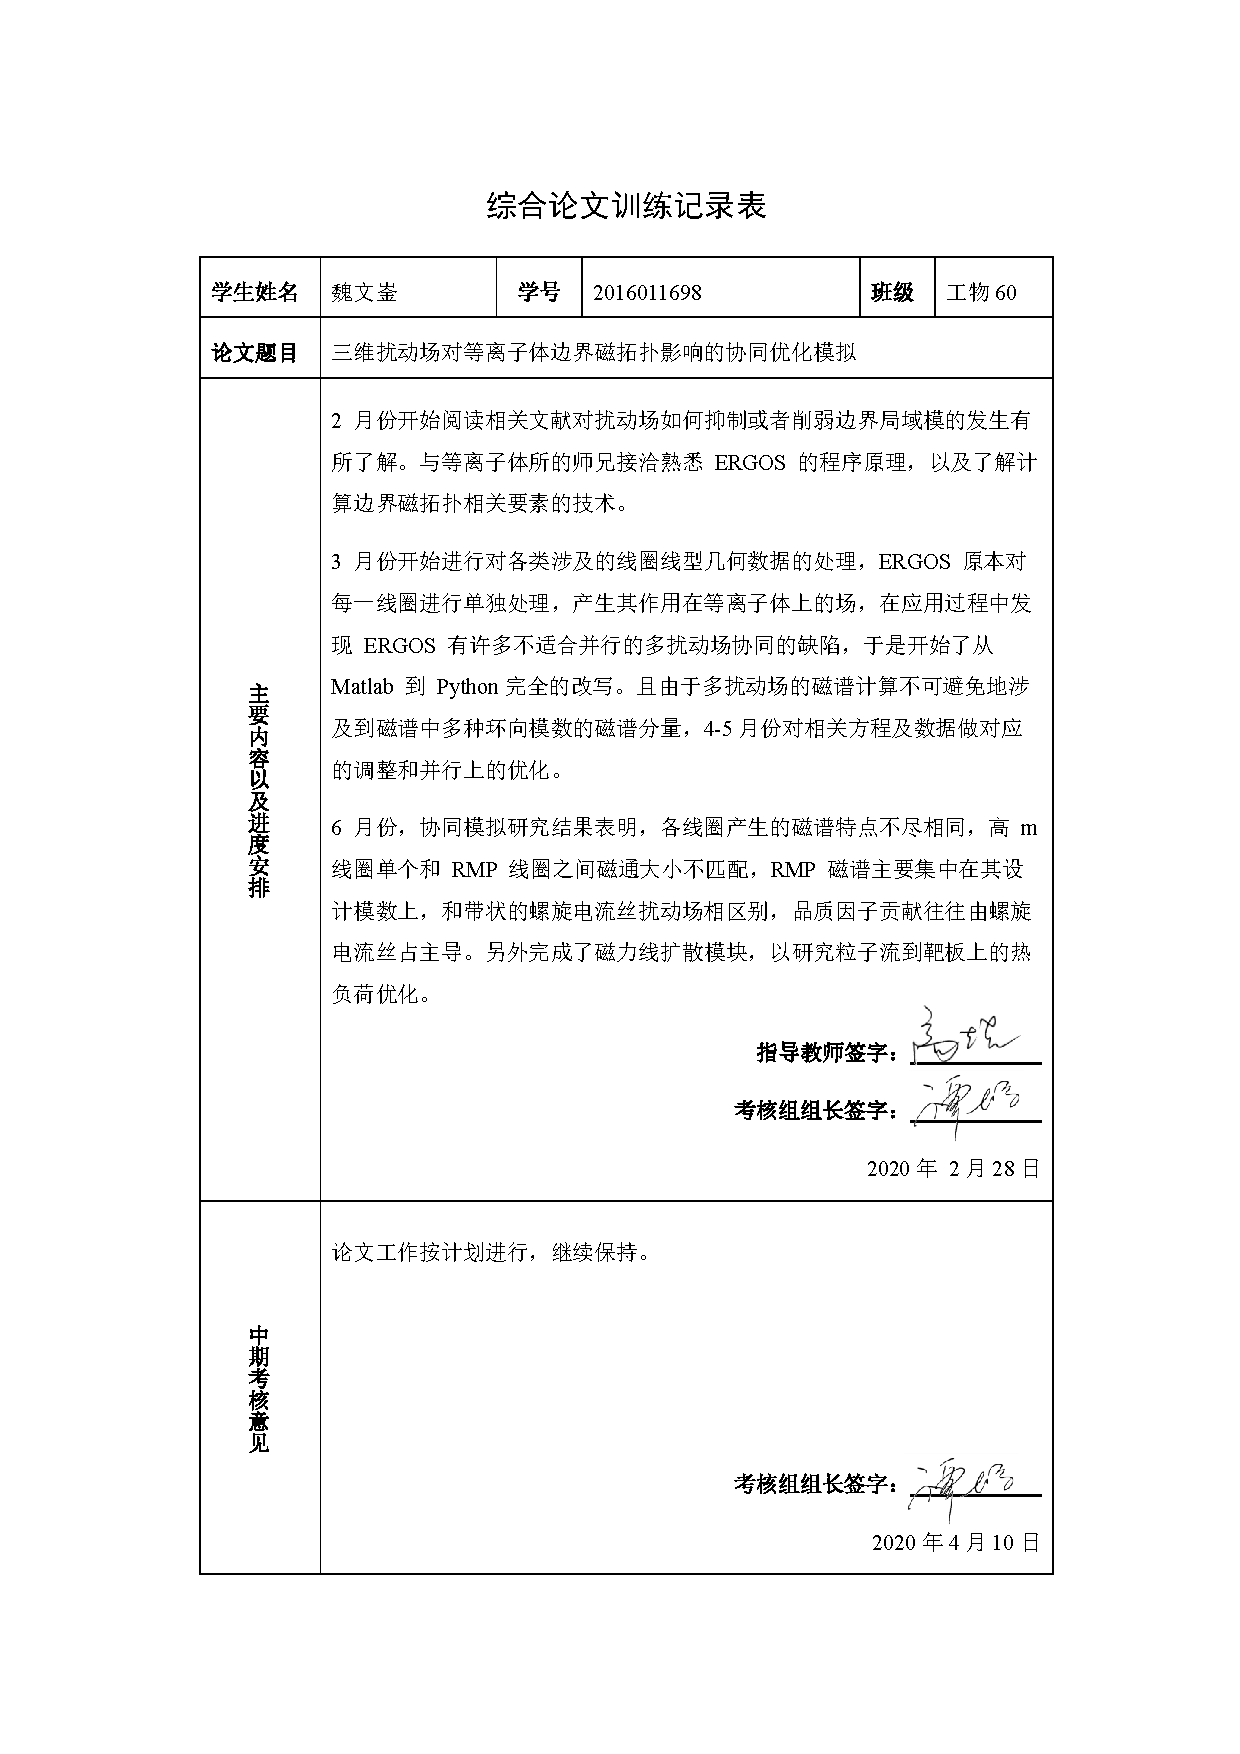
\includepdf[pages=-]{scan-record.pdf}
\end{document}
